\documentclass[aspectratio=169,12pt]{beamer}
\usepackage[utf8]{inputenc}
\usepackage{amsmath, amssymb}
\usepackage{booktabs}
\usepackage{colortbl}
\usepackage{hyperref}
\usepackage{makecell}
\usepackage{ragged2e}
\usepackage{bytefield}
\usepackage{tikz}
\usetikzlibrary{arrows.meta, positioning, shapes.geometric, calc, tikzmark, shapes.misc, matrix, backgrounds, fit, shadows, shapes.callouts}
\usepackage[siunitx]{circuitikz}
\usepackage{tcolorbox}
\usepackage[normalem]{ulem}
\usepackage{minted}
\setminted{fontsize=\footnotesize, breaklines}
\usetheme{Madrid}
\title{Hardware Security Mechanisms}
\author{Computer Architecture 2360267}
\date{2025, Lecture \#11}
\begin{document}
\frame{\titlepage}

% TODOs:
% Start with the security rings.
% When talking about SMAP, SMEP, need to somehow convey it's relevant for all high-level ring accessing arbitrary data of lower ring.
% Remove the "Homomorphic Encryption" stuff.
% Maybe something about the special "secutity chips" like apple's. Also "Security Processor (AMD-SP):" when talking about Intel ME.



% Outline
\begin{frame}{Outline}
    \tableofcontents
\end{frame}

% Additional slides to be inserted into the main presentation

% Section: Threat Model
\section{Threat Model}

\begin{frame}{Understanding Threat Models}
    \begin{columns}
        \begin{column}{0.5\textwidth}
            \textbf{What is a Threat Model?}
            \begin{itemize}
                \item Systematic analysis of:
                \begin{itemize}
                    \item What are we protecting?
                    \item Who are the attackers?
                    \item What capabilities do they have?
                    \item What are acceptable risks?
                \end{itemize}
            \end{itemize}
            
            \vspace{0.3cm}
            \textbf{Named Threat Models:}
            \begin{itemize}
                \item \textbf{Evil Maid:} Physical access when unattended
                \item \textbf{Honest but Curious:} Cloud provider with data access
                \item \textbf{Supply Chain:} Compromised hardware/firmware
            \end{itemize}
            
            \vspace{0.3cm}
            \textbf{Attacker Capabilities:}
            \begin{itemize}
                \item \textcolor{green!60!black}{User-level code execution}
                \item \textcolor{orange}{Memory corruption bugs}
                \item \textcolor{red}{Kernel vulnerabilities}
                \item \textcolor{red!80!black}{Physical access}
            \end{itemize}
        \end{column}
        \begin{column}{0.5\textwidth}
            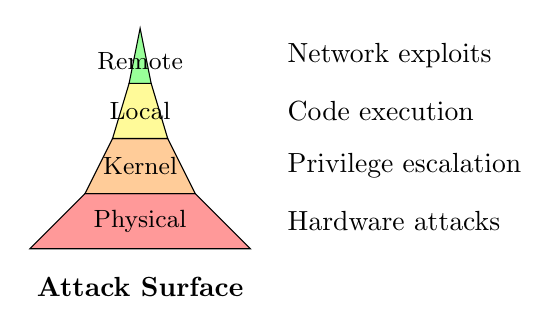
\begin{tikzpicture}[scale=0.7]
                % Threat levels pyramid
                \draw[fill=red!40] (0,0) -- (4,0) -- (3,1) -- (1,1) -- cycle;
                \node at (2,0.5) {\small Physical};
                
                \draw[fill=orange!40] (1,1) -- (3,1) -- (2.5,2) -- (1.5,2) -- cycle;
                \node at (2,1.5) {\small Kernel};
                
                \draw[fill=yellow!40] (1.5,2) -- (2.5,2) -- (2.2,3) -- (1.8,3) -- cycle;
                \node at (2,2.5) {\small Local};
                
                \draw[fill=green!40] (1.8,3) -- (2.2,3) -- (2,4) -- cycle;
                \node at (2,3.4) {\small Remote};
                
                % Labels
                \node[right] at (4.5,0.5) {Hardware attacks};
                \node[right] at (4.5,1.5) {Privilege escalation};
                \node[right] at (4.5,2.5) {Code execution};
                \node[right] at (4.5,3.5) {Network exploits};
                
                \node at (2,-0.7) {\textbf{Attack Surface}};
            \end{tikzpicture}
        \end{column}
    \end{columns}
    
    \vspace{0.5cm}
    \begin{tcolorbox}[colback=blue!10]
        \textbf{Modern CPU Security Mechanisms Target:}
        \begin{itemize}
            \item Memory corruption exploitation (buffer overflows, use-after-free)
            \item Control flow hijacking (ROP, JOP, code injection)
            \item Privilege escalation (kernel exploitation)
            \item Side-channel attacks (Spectre, Meltdown)
        \end{itemize}
    \end{tcolorbox}
\end{frame}

\begin{frame}{Defense in Depth}
    \begin{center}
        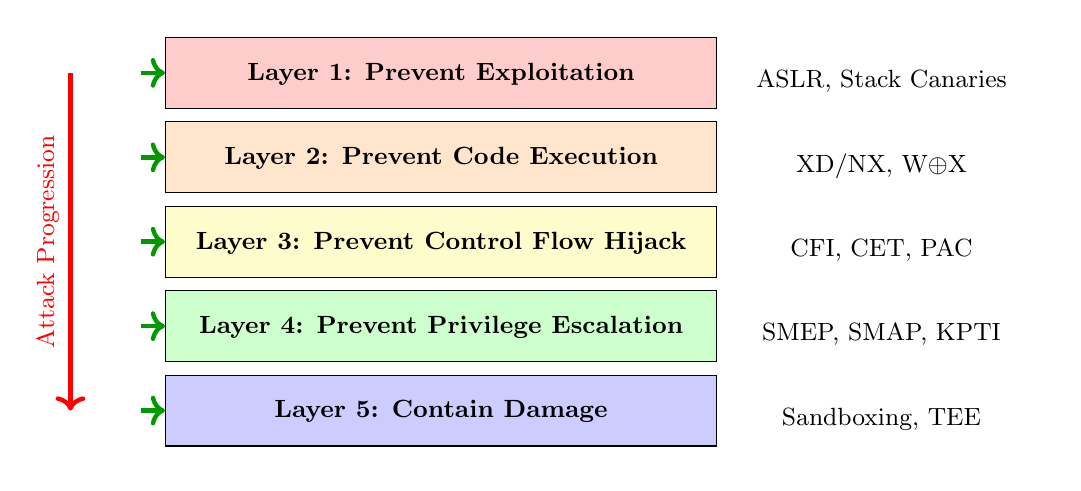
\begin{tikzpicture}[
            layer/.style={minimum height=0.9cm, text depth=0.2ex, font=\small},
            layer name/.style={layer, draw, minimum width=7cm},
            layer tech/.style={layer, minimum width=4cm, align=left, anchor=west}]

            \matrix[matrix of nodes, row sep=2pt, column sep=4pt,
                    ampersand replacement=\&, nodes={layer}] (m) {
                |[layer name, fill=red!20]| \textbf{Layer 1: Prevent Exploitation} \&
                |[layer tech]| ASLR, Stack Canaries \\
                |[layer name, fill=orange!20]| \textbf{Layer 2: Prevent Code Execution} \&
                |[layer tech]| XD/NX, W$\oplus$X \\
                |[layer name, fill=yellow!20]| \textbf{Layer 3: Prevent Control Flow Hijack} \&
                |[layer tech]| CFI, CET, PAC \\
                |[layer name, fill=green!20]| \textbf{Layer 4: Prevent Privilege Escalation} \&
                |[layer tech]| SMEP, SMAP, KPTI \\
                |[layer name, fill=blue!20]| \textbf{Layer 5: Contain Damage} \&
                |[layer tech]| Sandboxing, TEE \\
            };

            % Defense arrows
            \foreach \i in {1,...,5} {
                \draw[<-, ultra thick, green!60!black] (m-\i-1.west) -- ++(-0.3,0);
            }

            % Attack progression arrow - draw bottom to top so text reads upward, arrow points down
            \draw[<-, ultra thick, red] ([xshift=-1.2cm]m-5-1.west) -- ([xshift=-1.2cm]m-1-1.west)
                node[midway, sloped, above, red, font=\small] {Attack Progression};
        \end{tikzpicture}
    \end{center}

    \vspace{0.3cm}
    \begin{tcolorbox}[colback=yellow!20]
        \centering
        \textbf{Principle:} No single defense is perfect - multiple independent layers increase attack complexity exponentially
    \end{tcolorbox}
\end{frame}

% Section: Memory & Control Flow Security
\section{Memory \& Control Flow Security}
\subsection{ROP Protection}

\begin{frame}{Execute Disable (XD/NX) Bit - The First Line}
    \begin{columns}
        \begin{column}{0.5\textwidth}
            \textbf{XD/NX Bit Basics:}
            \begin{itemize}
                \item Intel: XD (eXecute Disable)
                \item AMD: NX (No eXecute)
                \item ARM: XN (eXecute Never)
                \item Page table bit 63
            \end{itemize}
            
            \vspace{0.3cm}
            \textbf{How it Works:}
            \begin{itemize}
                \item Marks memory pages non-executable
                \item CPU raises \#PF on exec attempt
                \item Enforces W$\oplus$X policy
            \end{itemize}
        \end{column}
        \begin{column}{0.5\textwidth}
            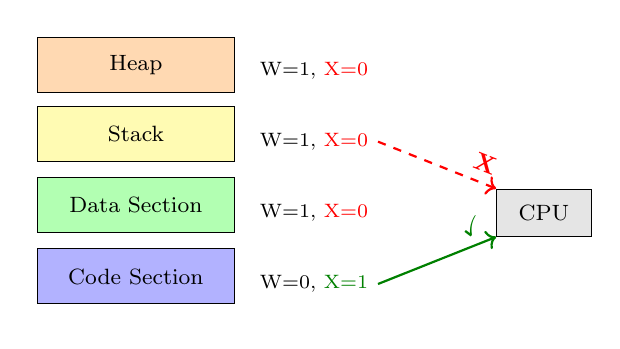
\begin{tikzpicture}[font=\footnotesize,
                mem section/.style={draw, minimum width=2.5cm, minimum height=0.7cm},
                perm/.style={minimum height=0.7cm, font=\scriptsize, anchor=west}]

                % Memory layout with permissions as second column
                \matrix[matrix of nodes, row sep=0.1cm, column sep=0.2cm,
                        ampersand replacement=\&] (mem) {
                    |[mem section, fill=orange!30]| Heap \&
                    |[perm]| W=1, \textcolor{red}{X=0} \\
                    |[mem section, fill=yellow!30]| Stack \&
                    |[perm]| W=1, \textcolor{red}{X=0} \\
                    |[mem section, fill=green!30]| Data Section \&
                    |[perm]| W=1, \textcolor{red}{X=0} \\
                    |[mem section, fill=blue!30]| Code Section \&
                    |[perm]| W=0, \textcolor{green!50!black}{X=1} \\
                };

                % CPU node
                \node[draw, fill=gray!20, minimum width=1.2cm, minimum height=0.6cm,
                      right=1.5cm of mem-3-2] (cpu) {CPU};

                % Execution arrow - only from Code Section (with checkmark)
                \draw[->, thick, green!50!black] (mem-4-2.east) -- (cpu.south west)
                    node[pos=0.85, above, font=\small, sloped] {\checkmark};

                % Blocked execution from Stack
                \draw[->, thick, red, dashed] (mem-2-2.east) -- (cpu.north west)
                    node[pos=0.85, above, font=\small\bfseries, sloped] {X};
            \end{tikzpicture}

            \vspace{0.3cm}
            \textbf{What XD Prevents:}
            \begin{itemize}
                \item Classic buffer overflow + shellcode
                \item Direct code injection attacks
            \end{itemize}
        \end{column}
    \end{columns}
\end{frame}

\begin{frame}{Why XD/NX is Not Enough - Enter ROP}
    \begin{columns}
        \begin{column}{0.5\textwidth}
            \textbf{The Problem:}
            \begin{itemize}
                \item Attackers don't need new code!
                \item Existing code has everything needed
                \item Chain existing code snippets
            \end{itemize}
            
            \vspace{0.3cm}
            \textbf{Return-Oriented Programming:}
            \begin{itemize}
                \item Uses "gadgets" ending in RET
                \item Gadget = useful instruction(s) + RET
                \item Chain gadgets via stack control
                \item Turing complete!
            \end{itemize}
        \end{column}
        \begin{column}{0.5\textwidth}
            \textbf{ROP Attack Example:} {\small(execve("/bin/sh"))}
            \vspace{-2mm}
            \begin{tcolorbox}[colback=gray!10, left=1mm, right=1mm, top=1mm, bottom=1mm]
                \ttfamily\scriptsize
                \begin{tabular}{@{}l@{\hspace{2mm}}l@{}}
                    \textbf{Stack:} & \textbf{Effect:} \\
                    {[}gadget1{]} & pop rdi; ret \\
                    {[}"/bin/sh"{]} & \textrm{\scriptsize$\rightarrow$ rdi = arg1} \\
                    {[}gadget2{]} & pop rsi; ret \\
                    {[}0{]} & \textrm{\scriptsize$\rightarrow$ rsi = arg2} \\
                    {[}gadget3{]} & mov rax,59; ret \\
                    & \textrm{\scriptsize$\rightarrow$ syscall \#} \\
                    {[}gadget4{]} & syscall \\
                \end{tabular}
            \end{tcolorbox}
            
            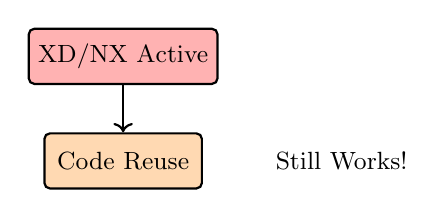
\begin{tikzpicture}[
                box/.style={draw, thick, minimum width=2cm, minimum height=0.7cm,
                           align=center, font=\small, rounded corners=2pt},
                arrow/.style={->, thick}]

                % XD/NX Active box at top
                \node[box, fill=red!30] (xd) {XD/NX Active};

                % Arrow pointing down
                \draw[arrow] (xd.south) -- ++(0, -0.6cm);

                % Code Reuse box below
                \node[box, fill=orange!30, below=0.6cm of xd] (reuse) {Code Reuse};

                % "Still Works!" annotation
                \node[font=\small, right=0.8cm of reuse] {Still Works!};
            \end{tikzpicture}
        \end{column}
    \end{columns}
\end{frame}

\begin{frame}{ROP Attack Visualization}
    \begin{center}
        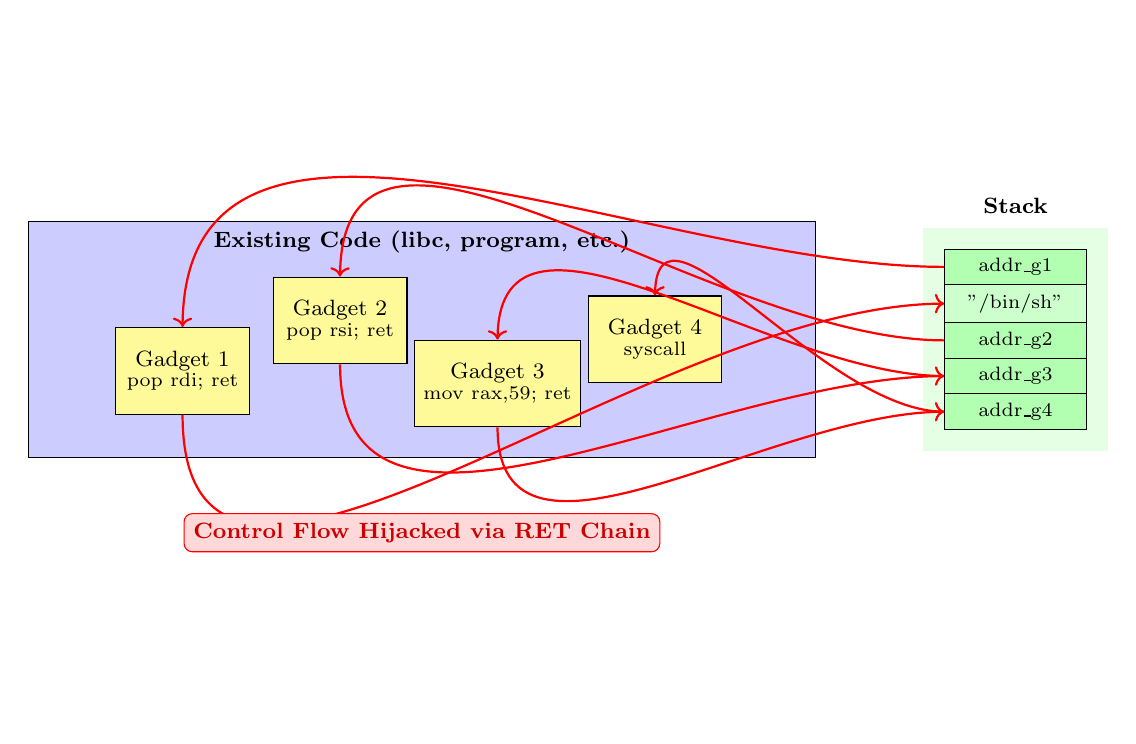
\begin{tikzpicture}[scale=0.8, font=\footnotesize,
            gadget/.style={draw, fill=yellow!40, minimum width=1.7cm, minimum height=1.1cm, align=center},
            stack cell/.style={draw, minimum width=1.8cm, minimum height=0.4cm, font=\scriptsize},
            flow/.style={->, thick, red}]

            % Code section background
            \node[draw, fill=blue!20, minimum width=10cm, minimum height=3cm] (code) at (5,1.5) {};
            \node[font=\footnotesize\bfseries, anchor=north] at (code.north) {Existing Code (libc, program, etc.)};

            % Gadgets - positioned within code section
            \node[gadget] (g1) at (1.2,1) {Gadget 1\\[-2pt]{\scriptsize pop rdi; ret}};
            \node[gadget] (g2) at (3.7,1.8) {Gadget 2\\[-2pt]{\scriptsize pop rsi; ret}};
            \node[gadget] (g3) at (6.2,0.8) {Gadget 3\\[-2pt]{\scriptsize mov rax,59; ret}};
            \node[gadget] (g4) at (8.7,1.5) {Gadget 4\\[-2pt]{\scriptsize syscall}};

            % Stack using matrix
            \matrix[matrix of nodes,
                nodes={stack cell},
                row sep=-\pgflinewidth,
                right=1.5cm of code] (stack) {
                |[fill=green!30]| addr\_g1 \\
                |[fill=green!20]| "/bin/sh" \\
                |[fill=green!30]| addr\_g2 \\
                |[fill=green!30]| addr\_g3 \\
                |[fill=green!30]| addr\_g4 \\
            };
            \node[font=\footnotesize\bfseries, above=0.2cm of stack] {Stack};

            % Background for stack
            \begin{scope}[on background layer]
                \node[fill=green!10, fit=(stack), inner sep=4pt] {};
            \end{scope}

            % Execution flow arrows
            \draw[flow] (stack-1-1.west) to[out=180,in=90] (g1.north);
            \draw[flow] (g1.south) to[out=-90,in=180] (stack-2-1.west);
            \draw[flow] (stack-3-1.west) to[out=180,in=90] (g2.north);
            \draw[flow] (g2.south) to[out=-90,in=180] (stack-4-1.west);
            \draw[flow] (stack-4-1.west) to[out=180,in=90] (g3.north);
            \draw[flow] (g3.south) to[out=-90,in=180] (stack-5-1.west);
            \draw[flow] (stack-5-1.west) to[out=180,in=90] (g4.north);

            % Caption
            \node[draw=red, fill=red!15, rounded corners=3pt, text=red!80!black, font=\footnotesize\bfseries, below=0.7cm of code] {Control Flow Hijacked via RET Chain};
        \end{tikzpicture}
    \end{center}

    \begin{tcolorbox}[colback=red!10]
        \textbf{Key Insight:} ROP bypasses XD/NX by reusing existing executable code - no code injection needed!
    \end{tcolorbox}
\end{frame}

% Protection Mechanisms in Detail
\begin{frame}<0>[fragile]{ASLR - Address Space Layout Randomization}
    \begin{columns}
        \begin{column}{0.5\textwidth}
            \textbf{How ASLR Works:}
            \begin{itemize}
                \item Randomizes memory addresses at runtime
                \item Different addresses each execution
                \item Makes hardcoded exploits fail
                \item Low performance overhead
            \end{itemize}
            
            \vspace{0.3cm}
            \textbf{What Gets Randomized:}
            \begin{itemize}
                \item Stack base address
                \item Heap base address
                \item Library load addresses
                \item Executable base (PIE)
                \item mmap region
            \end{itemize}
            
            \vspace{0.3cm}
            \textbf{Limitations:}
            \begin{itemize}
                \item Info leaks reveal addresses
                \item Partial overwrites still work
                \item Entropy limitations (32-bit)
            \end{itemize}
        \end{column}
        \begin{column}{0.5\textwidth}
            \vspace{-3cm}
            \begin{tcolorbox}[colback=green!10]
                \small
                \textbf{With ASLR (randomized):}
\begin{minted}[fontsize=\scriptsize]{console}
$ ./vuln
Stack: 0x7ffd8c3a1000
Heap:  0x56412b8c9000
Libc:  0x7f9a2c600000

$ ./vuln
Stack: 0x7ffe29f43000
Heap:  0x55e7d4521000
Libc:  0x7fc8e1200000
\end{minted}
            \end{tcolorbox}
        \end{column}
    \end{columns}
\end{frame}

\begin{frame}<0>[fragile]{Stack Canaries - Buffer Overflow Detection}
    \begin{columns}[T]
        \begin{column}{0.5\textwidth}
            \textbf{How Stack Canaries Work:}
            \begin{itemize}
                \item Random value placed before return address
                \item Checked before function returns
                \item Detects buffer overflows
                \item Compiler inserts automatically
            \end{itemize}
            
            \vspace{0.3cm}
            \textbf{Canary Types:}
            \begin{itemize}
                \item \textbf{Random:} From /dev/urandom
                \item \textbf{Terminator:} 0x00000aff
                \item \textbf{Random XOR:} Includes stack ptr
            \end{itemize}
        \end{column}
        \begin{column}{0.5\textwidth}
            \vspace{-7mm}
            \begin{tcolorbox}[colback=blue!10]
                \small
                \textbf{Vulnerable Function:}
\begin{minted}[fontsize=\scriptsize]{c}
void vulnerable(char *input) {
    char buffer[64];
    strcpy(buffer, input);
    return;
}
\end{minted}
            \end{tcolorbox}
            
            \begin{tcolorbox}[colback=green!10]
                \small
                \textbf{With Stack Canary:}
\begin{minted}[fontsize=\scriptsize]{nasm}
vulnerable:
    push rbp
    mov rbp, rsp
    sub rsp, 0x50

    ; Place canary
    mov rax, fs:[0x28]
    mov [rbp-0x8], rax

    ; Function body
    lea rdi, [rbp-0x48]
    call strcpy

    ; Check canary
    mov rax, [rbp-0x8]
    xor rax, fs:[0x28]
    jne .canary_fail

    leave
    ret

.canary_fail:
    call __stack_chk_fail
\end{minted}
            \end{tcolorbox}
        \end{column}
    \end{columns}
\end{frame}

\begin{frame}<0>[fragile]{Stack Canary - Memory Layout}
    \begin{center}
        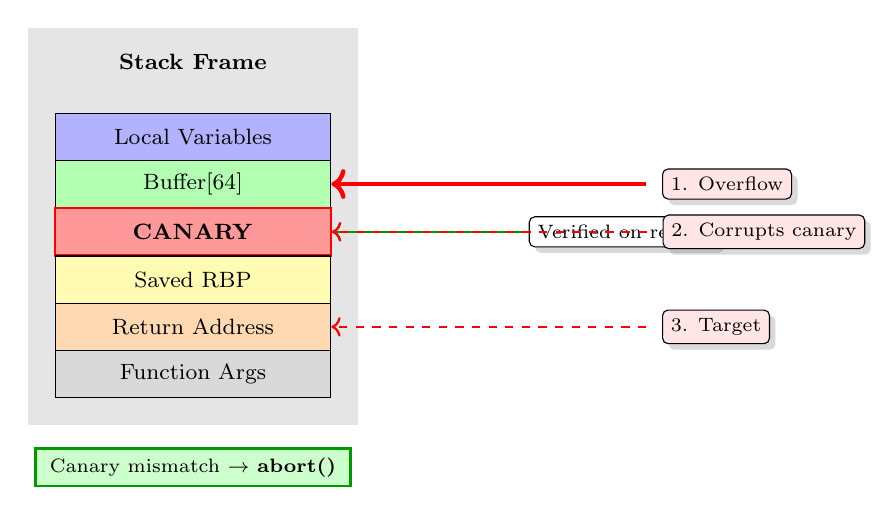
\begin{tikzpicture}[font=\footnotesize,
            stack cell/.style={draw, minimum width=3.5cm, minimum height=0.6cm},
            callout/.style={draw, fill=white, font=\scriptsize, rounded corners=2pt,
                           inner sep=3pt, drop shadow={opacity=0.3}}]

            % Stack frame title
            \node[font=\footnotesize\bfseries] (title) {Stack Frame};

            % Stack contents using matrix
            \matrix[matrix of nodes,
                nodes={stack cell},
                row sep=-\pgflinewidth,
                below=0.3cm of title] (stack) {
                |[fill=blue!30]| Local Variables \\
                |[fill=green!30]| Buffer[64] \\
                |[fill=red!40, draw=red, thick]| \textbf{CANARY} \\
                |[fill=yellow!30]| Saved RBP \\
                |[fill=orange!30]| Return Address \\
                |[fill=gray!30]| Function Args \\
            };

            % Background for stack frame
            \begin{scope}[on background layer]
                \node[fill=gray!20, fit=(title)(stack), inner sep=6pt] {};
            \end{scope}

            % Stage 1: Normal state - canary check annotation
            \node[callout, right=2.5cm of stack-3-1] (check) {Verified on return};
            \draw[->, thick, green!60!black] (check.west) -- (stack-3-1.east);

            % Stage 2: Overflow attack
            \onslide<2->{
                \draw[->, ultra thick, red] ([xshift=4cm]stack-2-1.east) -- (stack-2-1.east);
                \node[callout, fill=red!10, right=4.2cm of stack-2-1] (overflow) {1. Overflow};
            }

            % Stage 3: Canary corruption
            \onslide<3->{
                \draw[->, thick, red, dashed] ([xshift=4cm]stack-3-1.east) -- (stack-3-1.east);
                \node[callout, fill=red!10, right=4.2cm of stack-3-1] (corrupt) {2. Corrupts canary};
            }

            % Stage 4: Target and detection
            \onslide<4->{
                \draw[->, thick, red, dashed] ([xshift=4cm]stack-5-1.east) -- (stack-5-1.east);
                \node[callout, fill=red!10, right=4.2cm of stack-5-1] (target) {3. Target};
            }

            % Detection result
            \onslide<5->{
                \node[draw=green!60!black, fill=green!20, font=\scriptsize, thick,
                      below=0.5cm of stack, minimum width=4cm]
                    {Canary mismatch $\rightarrow$ \textbf{abort()}};
            }
        \end{tikzpicture}
    \end{center}
\end{frame}

% SMEP and SMAP (part of ROP Protection)

\begin{frame}{SMEP - Supervisor Mode Execution Prevention}
    \begin{columns}
        \begin{column}{0.55\textwidth}
            \textbf{ret2user Attack:}
            \begin{itemize}
                \item Kernel exploits redirect to user code
                \item User controls memory at known addresses
            \end{itemize}

            \vspace{0.3cm}
            \textbf{SMEP Solution:}
            \begin{itemize}
                \item CR4.SMEP bit (bit 20)
                \item Prevents kernel executing user pages
                \item \#PF if CPL=0 tries to execute U=1 page
                \item Intel: Ivy Bridge (2012)
            \end{itemize}
        \end{column}
        \begin{column}{0.45\textwidth}
            \centering
            \begin{tikzpicture}[
                space/.style={draw, thick, minimum width=2.8cm, minimum height=1.4cm,
                            align=center, font=\small, rounded corners=2pt},
                label/.style={draw, fill=white, rounded corners=2pt, font=\tiny,
                            inner sep=2pt}]

                % Kernel Space at top
                \node[space, fill=purple!15] (kernel) {};
                \node[font=\small, above=1mm of kernel.south] {\textbf{Kernel Space}};
                \node[label, below=1mm of kernel.north] {CPL = 0};

                % PTE bar in the middle
                \node[draw, thick, fill=yellow!30, minimum width=2.8cm, minimum height=0.5cm,
                      below=0.7cm of kernel, font=\scriptsize] (pte) {PTE: U = 1};

                % User Space at bottom
                \node[space, fill=cyan!10, below=0.7cm of pte] (user) {};
                \node[font=\small, above=1mm of user.south] {\textbf{User Space}};
                \node[font=\scriptsize, fill=red!20, rounded corners=2pt,
                      inner sep=2pt, below=1mm of user.north] {Shellcode};

                % Code annotation and attack arrow from kernel center
                \draw[->, thick, red, dashed] (kernel.south) -- (pte.north)
                    node[font=\ttfamily\tiny, red, midway, left=1mm] {jmp *\%rax};
                \draw[->, thick, red, dashed] (pte.south) -- (user.north);

                % Block symbol and label together
                \node[inner sep=0pt, right=3mm of pte.east] (xmark)
                    {\includegraphics[width=0.45cm]{figures/noun-x-2222229.png}};
                \node[red, font=\scriptsize, below=0mm of xmark] {SMEP};
            \end{tikzpicture}
        \end{column}
    \end{columns}

    \vspace{0.3cm}
    \begin{tcolorbox}[colback=yellow!20]
        \textbf{Bypass Methods:} ROP in kernel code, physmap spraying
    \end{tcolorbox}
\end{frame}

\begin{frame}[fragile]{SMAP - Supervisor Mode Access Prevention}
    \begin{columns}
        \begin{column}{0.5\textwidth}
            \textbf{The Problem After SMEP:}
            \begin{itemize}
                \item Can't execute user pages
                \item But can still READ/WRITE them!
                \item Kernel ROP can use user data
                \item Arbitrary write to user buffers
            \end{itemize}
            
            \vspace{0.3cm}
            \textbf{SMAP Solution:}
            \begin{itemize}
                \item CR4.SMAP bit (bit 21)
                \item Blocks kernel access to user pages
                \item STAC/CLAC instructions for legitimate access
                \item Intel: Broadwell (2014)
            \end{itemize}
        \end{column}
        \begin{column}{0.5\textwidth}
            \textbf{Kernel Code Pattern:}
            \vspace{-2mm}
            \begin{tcolorbox}[colback=gray!10, left=1mm, right=1mm, top=1mm, bottom=1mm]
\begin{minted}[fontsize=\scriptsize]{gas}
copy_from_user:
    STAC        ; Enable access
    mov (%rdi), %rax
    CLAC        ; Disable access
    ret

; Vulnerability example:
some_ioctl:
    ; Missing STAC/CLAC!
    mov %rsi, (%rdi)  ; Oops!
\end{minted}
            \end{tcolorbox}
            
            \textbf{EFLAGS.AC bit:}
            \begin{itemize}
                \item AC=0: SMAP active (default)
                \item AC=1: Temporary user access
                \item Only changeable in Ring 0
            \end{itemize}
        \end{column}
    \end{columns}
\end{frame}

% Subsection: Memory Protection
\subsection{Memory Protection}

\begin{frame}{Pointer Tagging - Using Unused Pointer Bits}
    \begin{columns}
        \begin{column}{0.5\textwidth}
            \textbf{Concept:}
            \begin{itemize}
                \item 64-bit pointers only use 48 bits for address
                \item Upper 16 bits available for metadata
                \item Hardware can check metadata on access
            \end{itemize}

            \vspace{0.3cm}
            \textbf{Two Security Applications:}
            \vspace{0.2cm}

            \colorbox{green!20}{\textbf{Memory Safety (MTE):}}
            \begin{itemize}
                \item Tag memory regions with colors
                \item Detect use-after-free, overflows
            \end{itemize}

            \vspace{0.2cm}
            \colorbox{blue!20}{\textbf{Control Flow (PAC):}}
            \begin{itemize}
                \item Cryptographic pointer signatures
                \item Protect return addresses, function ptrs
            \end{itemize}
        \end{column}
        \begin{column}{0.5\textwidth}
            \centering
            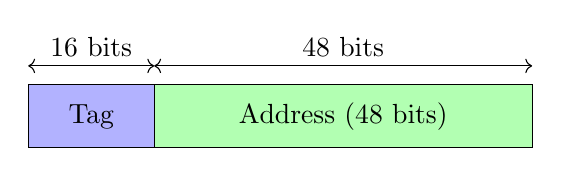
\begin{tikzpicture}[scale=0.8]
                \draw (0,0) rectangle (8,1);
                \draw[fill=blue!30] (0,0) rectangle (2,1);
                \draw[fill=green!30] (2,0) rectangle (8,1);
                \node at (1,0.5) {Tag};
                \node at (5,0.5) {Address (48 bits)};
                \draw[<->] (0,1.3) -- (2,1.3) node[midway,above] {16 bits};
                \draw[<->] (2,1.3) -- (8,1.3) node[midway,above] {48 bits};
            \end{tikzpicture}

            \vspace{0.5cm}
            \begin{tcolorbox}[colback=yellow!10]
                \small
                \textbf{Same mechanism, different goals:}\\[2pt]
                MTE $\rightarrow$ \textit{Where} can I access?\\
                PAC $\rightarrow$ \textit{Where} can code jump?
            \end{tcolorbox}
        \end{column}
    \end{columns}
\end{frame}

\begin{frame}{ARM MTE - Memory Safety via Tagging}
    \begin{columns}
        \begin{column}{0.49\textwidth}
            \textbf{Memory Granularity:}
            \begin{itemize}
                \item Each 16-byte memory granule has a 4-bit tag
                \item Tags stored in dedicated tag memory
                \item Tag memory not directly accessible
            \end{itemize}

            %\vspace{0.3cm}
            \textbf{Hardware Tag Checking:}
            \begin{itemize}
                \item On every load/store: compare pointer tag with memory tag
                \item If mismatch $\rightarrow$ exception
                \item \textbf{Probabilistic:} 4-bit tag = 1/16 chance of collision
            \end{itemize}

            %\vspace{0.3cm}
        \end{column}
        \begin{column}{0.49\textwidth}
            \textbf{Key Instructions:}
            \begin{itemize}
                \item \texttt{IRG} -- Insert Random tag into pointer
                \item \texttt{STG} -- Store Allocation Tag to memory
                \item \texttt{LDG} -- Load Allocation Tag from memory
            \end{itemize}

            \vspace{0.3cm}
            \textbf{Allocator Integration:}
            \begin{itemize}
                \item \texttt{malloc()}: uses \texttt{IRG} + \texttt{STG}
                \item \texttt{free()}: uses \texttt{STG} with new tag
                \item Hardware checks tag on every access
            \end{itemize}

            \vspace{0.3cm}
            {\small \textbf{Note:} Probabilistic detection ($\sim$94\% per access)}
        \end{column}
    \end{columns}
\end{frame}

\begin{frame}{ARM MTE - Detecting Memory Errors}
    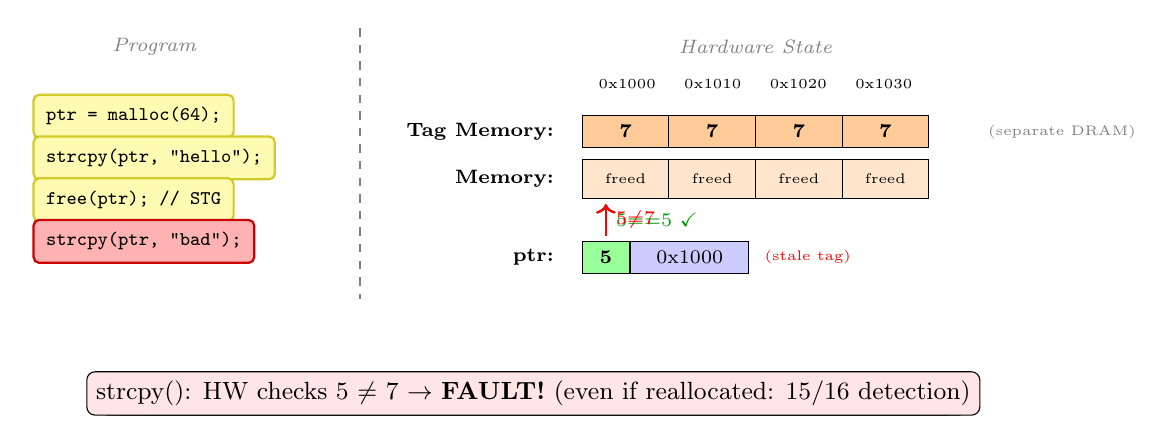
\begin{tikzpicture}[
        memcell/.style={draw, minimum width=1.1cm, minimum height=0.5cm, font=\tiny},
        tagcell/.style={draw, minimum width=1.1cm, minimum height=0.4cm, font=\scriptsize\bfseries},
        codeline/.style={font=\ttfamily\scriptsize, anchor=west},
        highlight/.style={draw=yellow!80!black, fill=yellow!30, thick, rounded corners=2pt},
        highlight bad/.style={draw=red!80!black, fill=red!30, thick, rounded corners=2pt},
        rowlabel/.style={font=\scriptsize\bfseries, anchor=east},
        ptrtag/.style={draw, minimum width=0.6cm, minimum height=0.4cm, font=\scriptsize\bfseries},
        ptrval/.style={draw, minimum width=1.5cm, minimum height=0.4cm, font=\scriptsize},
        allocated/.style={fill=green!40},
        freed/.style={fill=orange!40},
        allocmem/.style={fill=green!20},
        freedmem/.style={fill=orange!20},
        result/.style={draw=red, fill=red!20, thick, font=\small\bfseries, rounded corners=3pt}]

        % Code listing (left side)
        \matrix[matrix of nodes, nodes={codeline}, row sep=2pt] (code) {
            |(c1)| ptr = malloc(64); \\
            |(c2)| strcpy(ptr, "hello"); \\
            |(c3)| free(ptr); // STG \\
            |(c4)| strcpy(ptr, "bad"); \\
        };

        % Highlight current line (on background layer so code stays visible)
        \begin{scope}[on background layer]
            \onslide<1>{\node[highlight, fit=(c1), inner sep=1pt] {};}
            \onslide<2>{\node[highlight, fit=(c2), inner sep=1pt] {};}
            \onslide<3>{\node[highlight, fit=(c3), inner sep=1pt] {};}
            \onslide<4-5>{\node[highlight bad, fit=(c4), inner sep=1pt] {};}
        \end{scope}

        % Right side - memory visualization
        % Tag Memory (separate storage) with address labels above
        \node[rowlabel] (taglabel) at (5.2, 0.6) {Tag Memory:};
        \matrix[matrix of nodes,
            nodes={tagcell, fill=gray!20},
            column sep=-\pgflinewidth,
            ampersand replacement=\&,
            right=3pt of taglabel.east, anchor=west] (tags) {
            - \& - \& - \& - \\
        };
        % Address labels above tag cells (no border/background)
        \matrix[matrix of nodes,
            nodes={font=\tiny, minimum width=1.1cm, minimum height=0.3cm, inner sep=0pt},
            column sep=-\pgflinewidth,
            ampersand replacement=\&,
            anchor=south] at (tags.north) {
            0x1000 \& 0x1010 \& 0x1020 \& 0x1030 \\
        };

        % Color the tag cells based on state
        \onslide<1-2>{
            \node[tagcell, allocated] at (tags-1-1) {5};
            \node[tagcell, allocated] at (tags-1-2) {5};
            \node[tagcell, allocated] at (tags-1-3) {5};
            \node[tagcell, allocated] at (tags-1-4) {5};
        }
        \onslide<3->{
            \node[tagcell, freed] at (tags-1-1) {7};
            \node[tagcell, freed] at (tags-1-2) {7};
            \node[tagcell, freed] at (tags-1-3) {7};
            \node[tagcell, freed] at (tags-1-4) {7};
        }

        % Main Memory - label aligned to taglabel, matrix aligned to tags
        \node[rowlabel, below=0.6cm of taglabel.east, anchor=east] (memlabel) {Memory:};
        \matrix[matrix of nodes,
            nodes={memcell, fill=gray!10},
            column sep=-\pgflinewidth,
            ampersand replacement=\&,
            anchor=west] (mem) at (tags.west |- memlabel) {
            --- \& --- \& --- \& --- \\
        };

        % Color memory based on state - show content, not addresses
        \onslide<1>{
            \node[memcell, allocmem] at (mem-1-1) {---};
            \node[memcell, allocmem] at (mem-1-2) {---};
            \node[memcell, allocmem] at (mem-1-3) {---};
            \node[memcell, allocmem] at (mem-1-4) {---};
        }
        \onslide<2>{
            \node[memcell, allocmem] at (mem-1-1) {"hel};
            \node[memcell, allocmem] at (mem-1-2) {lo"};
            \node[memcell, allocmem] at (mem-1-3) {---};
            \node[memcell, allocmem] at (mem-1-4) {---};
        }
        \onslide<3->{
            \node[memcell, freedmem] at (mem-1-1) {freed};
            \node[memcell, freedmem] at (mem-1-2) {freed};
            \node[memcell, freedmem] at (mem-1-3) {freed};
            \node[memcell, freedmem] at (mem-1-4) {freed};
        }

        % Pointer variable - label aligned to memlabel, larger gap from Memory row
        \node[rowlabel, below=1cm of memlabel.east, anchor=east] (ptrlabel) {ptr:};
        % Pointer shown from stage 1 (after malloc)
        \node[ptrtag, allocated, anchor=west] (ptrtag-alloc) at (mem-1-1.west |- ptrlabel) {5};
        \node[ptrval, fill=blue!20, anchor=west] (ptrval-alloc) at (ptrtag-alloc.east) {0x1000};

        \onslide<3->{
            \node[font=\tiny, red, right=2pt of ptrval-alloc.east] {(stale tag)};
        }

        % Tag comparison visualization
        \onslide<2>{
            \draw[->, thick, green!60!black] ([yshift=2pt]ptrtag-alloc.north) -- ++(0, 0.4)
                node[right, font=\scriptsize, pos=0.5] {5==5 \checkmark};
        }
        \onslide<4->{
            \draw[->, thick, red] ([yshift=2pt]ptrtag-alloc.north) -- ++(0, 0.4)
                node[right, font=\scriptsize, pos=0.5] {5$\neq$7};
        }

        % Labels for sections
        \node[font=\scriptsize\itshape, gray, above=0.3cm of code.north] (proglabel) {Program};
        \node[font=\scriptsize\itshape, gray] at (tags.north |- proglabel) {Hardware State};

        % Separator line - from above program label to below ptr
        \draw[gray, dashed] ([xshift=1cm]proglabel.north -| code.east) -- ([xshift=1cm, yshift=-0.3cm]ptrlabel.south -| code.east);

        % Note about tag memory
        \node[font=\tiny, gray, anchor=west] at ([xshift=0.5cm]tags.east) {(separate DRAM)};

        % Description box at bottom center - use separate overlaid nodes
        \coordinate (descpos) at ([yshift=-1.5cm]ptrlabel.south);
        \onslide<1>{\node[draw, fill=blue!10, rounded corners=3pt, font=\small, minimum width=10cm] at (descpos) {malloc(64): Allocates memory, assigns tag 5 to both pointer and memory};}
        \onslide<2>{\node[draw, fill=green!10, rounded corners=3pt, font=\small, minimum width=10cm] at (descpos) {strcpy(): Hardware checks pointer tag (5) == memory tag (5) \checkmark};}
        \onslide<3>{\node[draw, fill=orange!10, rounded corners=3pt, font=\small, minimum width=10cm] at (descpos) {free() uses \texttt{STG} instruction to set memory tag to 7; pointer keeps stale tag 5};}
        \onslide<4-5>{\node[draw, fill=red!10, rounded corners=3pt, font=\small, minimum width=10cm] at (descpos) {strcpy(): HW checks 5 $\neq$ 7 $\rightarrow$ \textbf{FAULT!} (even if reallocated: 15/16 detection)};}
    \end{tikzpicture}
\end{frame}

\begin{frame}{Control Flow Integrity (CFI) - Overview}
    \begin{columns}
        \begin{column}{0.7\textwidth}
            \begin{itemize}
                \item Enforce legitimate control flow transfers
                \item Prevent code-reuse attacks (ROP/JOP/COP)
                \item Hardware + software enforcement
            \end{itemize}
            
            \vspace{0.3cm}
            \colorbox{green!20}{\textbf{Forward-Edge CFI:}}
            \begin{itemize}
                \item Indirect calls (call rax)
                \item Indirect jumps (jmp rbx)
                \item Virtual function calls
            \end{itemize}
            
            \colorbox{blue!20}{\textbf{Backward-Edge CFI:}}
            \begin{itemize}
                \item Function returns (ret)
                \item Return address integrity
            \end{itemize}
        \end{column}
        \begin{column}{0.3\textwidth}
            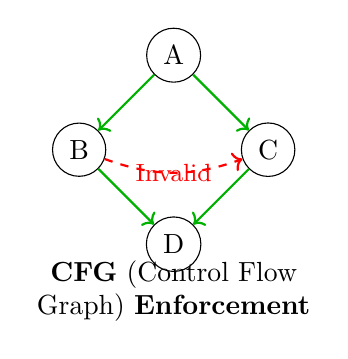
\begin{tikzpicture}[scale=0.6]
                % Control flow graph
                \node[draw,circle] (A) at (2,4) {A};
                \node[draw,circle] (B) at (0,2) {B};
                \node[draw,circle] (C) at (4,2) {C};
                \node[draw,circle] (D) at (2,0) {D};
                
                % Valid edges (green)
                \draw[->,thick,green!70!black] (A) -- (B);
                \draw[->,thick,green!70!black] (A) -- (C);
                \draw[->,thick,green!70!black] (B) -- (D);
                \draw[->,thick,green!70!black] (C) -- (D);
                
                % Invalid edge (red, dashed)
                \draw[->,thick,red,dashed] (B) to[bend right=20] (C);
                \node[red] at (2,1.5) {\small Invalid};
                
                \node[align=center] at (2,-1) {\textbf{CFG} (Control Flow\\Graph) \textbf{Enforcement}};
            \end{tikzpicture}
            
            \vspace{-2mm}
            \begin{tcolorbox}[colback=yellow!10]
                \small
                \textbf{Attack Example:}
                Attacker overwrites function pointer to jump from B→C, violating intended control flow
            \end{tcolorbox}
        \end{column}
    \end{columns}
\end{frame}
\begin{frame}[fragile]{Pointer Authentication (PAC) - Control Flow Protection}
    \begin{columns}
        \begin{column}{0.5\textwidth}
            \textbf{ARM PAC Architecture:}
            \begin{itemize}
                \item Cryptographic signature stored in upper pointer bits
                \item Uses QARMA block cipher
                \item 5 128-bit keys (IA, IB, DA, DB, GA)
            \end{itemize}
            
            \vspace{0.3cm}
            \textbf{Operations:}
            \begin{itemize}
                \item \texttt{PACIA}: Sign instruction pointer
                \item \texttt{AUTIA}: Authenticate pointer
                \item \texttt{PACDA}: Sign data pointer
            \end{itemize}
        \end{column}
        \begin{column}{0.5\textwidth}
            \textbf{Function Prologue:}
            \vspace{-2mm}
            \begin{tcolorbox}[colback=gray!10, left=1mm, right=1mm, top=1mm, bottom=1mm]
\begin{minted}[fontsize=\scriptsize]{gas}
; LR (x30) = return addr, SP = stack ptr
PACIASP    ; Sign LR using SP as context
STP x29,x30,[sp,#-16]!  ; Save frame ptr & LR
\end{minted}
            \end{tcolorbox}

            \vspace{-1mm}
            \textbf{Function Epilogue:}
            \vspace{-2mm}
            \begin{tcolorbox}[colback=gray!10, left=1mm, right=1mm, top=1mm, bottom=1mm]
\begin{minted}[fontsize=\scriptsize]{gas}
LDP x29,x30,[sp],#16    ; Restore frame ptr & LR
AUTIASP    ; Verify LR signature
RET        ; Return if valid, else fault
\end{minted}
            \end{tcolorbox}

            \vspace{2mm}
            \textbf{Security:} Prevents ROP/JOP attacks by cryptographically signing return addresses
        \end{column}
    \end{columns}
\end{frame}

% Subsection: Control Flow Integrity
\subsection{Control Flow Integrity}


\begin{frame}[fragile]{Forward-Edge CFI: Intel CET-IBT \& ARM BTI}
    \begin{columns}
        \begin{column}{0.6\textwidth}
            \textbf{Intel CET-IBT (Indirect Branch Tracking):}
            \begin{itemize}
                \item \texttt{ENDBRANCH} instruction marks valid targets
                \item CPU tracks indirect branch state
                \item Fault if target lacks \texttt{ENDBRANCH}
            \end{itemize}
            
            \vspace{0.3cm}
            \textbf{ARM BTI (Branch Target Identification):}
            \begin{itemize}
                \item \texttt{BTI} instructions mark valid targets
                \item Variants match branch types:
                \begin{itemize}
                    \item \texttt{BTI c}: Call target (BLR)
                    \item \texttt{BTI j}: Jump target (BR)
                    \item \texttt{BTI jc}: Both call \& jump
                \end{itemize}
                \item CPU faults on mismatch
            \end{itemize}
            
            %\vspace{0.3cm}
            %\textbf{Software CFI (LLVM):}
            %\begin{itemize}
            %    \item Type-based: Check function signatures
            %    \item Fine-grained: Unique IDs per callsite
            %    \item Cross-DSO support
            %\end{itemize}
        \end{column}
        \begin{column}{0.4\textwidth}
            \textbf{Example: Intel CET-IBT}
            \vspace{-2mm}
            \begin{tcolorbox}[colback=gray!10, left=1mm, right=1mm, top=1mm, bottom=1mm]
\begin{minted}[fontsize=\scriptsize]{nasm}
valid_target:
    endbranch    ; Mark as valid
    push rbp
    mov rbp, rsp
    ; Function body

invalid_target:  ; No endbranch
    push rbp     ; CPU fault here!
    mov rbp, rsp
\end{minted}
            \end{tcolorbox}
            
            \textbf{Protection Granularity:}
            \begin{itemize}
                \item \textbf{HW (coarse):} Any marked target
                \item \textbf{SW (fine):} Type-compatible
                \item \textbf{SW (ultra-fine):} Exact callsite
            \end{itemize}
        \end{column}
    \end{columns}
\end{frame}

\begin{frame}<0>[fragile]{ARM BTI Explained}
    \begin{columns}
        \begin{column}{0.5\textwidth}
            \textbf{BTI Instruction Variants:}
            \begin{itemize}
                \item \textbf{BTI c}: Target of calls (BLR/BLRA)
                \item \textbf{BTI j}: Target of jumps (BR/BRA)
                \item \textbf{BTI jc}: Target of both
                \item \textbf{BTI}: Same as BTI jc (alias)
            \end{itemize}
            
            \vspace{0.3cm}
            \textbf{How It Works:}
            \begin{enumerate}
                \item Indirect branch sets PSTATE.BTYPE
                \item Target instruction checked
                \item Must be correct BTI variant
                \item Otherwise: exception generated
            \end{enumerate}
            
            \vspace{0.3cm}
            \textbf{Use Cases:}
            \begin{itemize}
                \item Function entry points: BTI c
                \item Switch jump tables: BTI j
                \item PLT stubs: BTI jc
            \end{itemize}
        \end{column}
        \begin{column}{0.5\textwidth}
            \vspace{-7mm}
            \textbf{BTI Usage Example:}
            \vspace{-2mm}
            \begin{tcolorbox}[colback=gray!10, left=1mm, right=1mm, top=1mm, bottom=1mm]
\begin{minted}[fontsize=\scriptsize]{gas}
; Function called via pointer
func_ptr:
    BTI c      ; Mark as call target
    stp x29, x30, [sp, #-16]!
    ; Function body
    ldp x29, x30, [sp], #16
    ret

; Jump table target
case_handler:
    BTI j      ; Mark as jump target
    ; Handle case
    ret

; PLT stub (can be called or jumped to)
plt_stub:
    BTI jc     ; Both call and jump
    adrp x16, GOT_ENTRY
    ldr x17, [x16, #:lo12:GOT_ENTRY]
    br x17
\end{minted}
            \end{tcolorbox}
        \end{column}
    \end{columns}
\end{frame}

\begin{frame}<0>[fragile]{Pointer Authentication (PAC) - ARM64}
    \begin{columns}
        \begin{column}{0.5\textwidth}
            \textbf{How PAC Works:}
            \begin{itemize}
                \item Signs pointers with cryptographic MAC
                \item Uses upper bits (unused in 64-bit)
                \item Hardware acceleration (QARMA)
                \item 5 different keys (IA, IB, DA, DB, GA)
            \end{itemize}
            
            \vspace{0.3cm}
            \textbf{PAC Instructions:}
            \begin{itemize}
                \item \textbf{PACIA:} Sign with key A
                \item \textbf{AUTIA:} Authenticate with key A
                \item \textbf{PACIASP:} Sign with SP as context
                \item \textbf{AUTIASP:} Auth with SP as context
            \end{itemize}
            
            \vspace{0.3cm}
            \textbf{Protection Against:}
            \begin{itemize}
                \item ROP/JOP attacks
                \item Return address corruption
                \item Function pointer hijacking
            \end{itemize}
        \end{column}
        \begin{column}{0.5\textwidth}
            \vspace{-7mm}
            \begin{tcolorbox}[colback=green!10, left=1mm, right=1mm, top=1mm, bottom=1mm]
\begin{minted}[fontsize=\scriptsize]{gas}
sensitive_function:
    paciasp          ; Sign return address
    ; Save frame
    stp x29, x30, [sp, #-16]!
    mov x29, sp
    ; Function body ...
    ; Restore frame
    ldp x29, x30, [sp], #16
    ; Authenticate return address
    autiasp
    ; Return (crashes if auth fails)
    ret
\end{minted}
            \end{tcolorbox}

            \begin{tcolorbox}[colback=yellow!10]
                \small
                \textbf{Pointer Format:}
\begin{minted}[fontsize=\scriptsize]{text}
[63:56][55:48][47:0]
  PAC   Unused  Address
\end{minted}
            \end{tcolorbox}
        \end{column}
    \end{columns}
\end{frame}


\begin{frame}[fragile]{The Type Confusion Problem}
    \begin{columns}
        \begin{column}{0.6\textwidth}
            \textbf{What is Type Confusion?}
            \begin{itemize}
                \item Object interpreted as wrong type
                \item Enables control flow hijacking
                \item Bypass basic CFI checks
            \end{itemize}

            \vspace{0.15cm}
            \textbf{Attack Scenario:}
            \begin{itemize}
                \item Attacker controls object allocation
                \item Forces type confusion via UAF/overflow
                \item Calls virtual function on wrong type
                \item Jumps to attacker-controlled vtable
            \end{itemize}

            \vspace{0.15cm}
            \textbf{Why Basic CFI Fails:}
            \begin{itemize}
                \item All virtual calls are "valid" targets
                \item Cannot distinguish object types
            \end{itemize}
        \end{column}
        \begin{column}{0.4\textwidth}
            \begin{tcolorbox}[colback=gray!10, left=0mm, right=0mm, top=0mm, bottom=0mm]
\begin{minted}[fontsize=\scriptsize]{c}
void evil() { system("/bin/sh"); }

struct Object {
  void (*callback)(); // func ptr
  int data;
};
struct Input {
  char buffer[16];  // attacker input
};

// Type confusion: Input as Object
struct Input* in = get_input();
struct Object* obj = (Object*)in;

// Hijack! buffer interpreted as
// function pointer -> calls evil()
obj->callback();
\end{minted}
            \end{tcolorbox}
        \end{column}
    \end{columns}
\end{frame}

\begin{frame}[fragile]{FineIBT - Advanced Forward-Edge CFI}
    \begin{columns}
        \begin{column}{0.5\textwidth}
            \textbf{Linux Kernel Implementation:}
            \begin{itemize}
                \item Combines Intel CET-IBT with kCFI
                \item Function type hash validation
                \item Per-function-signature protection
            \end{itemize}
            
            \vspace{0.1cm}
            \textbf{How it Works:}
            \begin{enumerate}
                \item Compiler generates type hash
                \item Hash checked at indirect call site
                \item ENDBRANCH validates branch target
                \item Mismatch triggers exception
            \end{enumerate}
            
            \vspace{0.1cm}
            \textbf{Benefits over Basic IBT:}
            \begin{itemize}
                \item Type safety enforcement
                \item Prevents type confusion attacks
            \end{itemize}
        \end{column}
        \begin{column}{0.5\textwidth}
            \begin{tcolorbox}[colback=gray!10, left=1mm, right=1mm, top=1mm, bottom=1mm]
\begin{minted}[fontsize=\scriptsize]{gas}
; Caller: indirect call through %rax
    mov $0x12345678, %r11d ; Expected hash
    call *%rax             ; Indirect call

; Callee: func
func:
    endbranch              ; CET check
    sub $0x12345678, %r11d ; Compare hashes
    je .Lok                ; Match -> continue
    ud2                    ; Mismatch -> trap
.Lok:
    push rbp
    ; Function body
\end{minted}
            \end{tcolorbox}
            
            \begin{tcolorbox}[colback=yellow!10]
                \small
                \textbf{Attack Prevention:}
                Even if attacker finds valid ENDBRANCH target, type hash must also match
            \end{tcolorbox}
        \end{column}
    \end{columns}
\end{frame}

% Section: Hardware Isolation
\section{Hardware Isolation}
\subsection{Privilege Levels \& Virtualization}

\begin{frame}[fragile]{Shadow Stack - Hardware Return Address Protection}
    \begin{columns}
        \begin{column}{0.5\textwidth}
            \textbf{Shadow Stack Concept:}
            \begin{itemize}
                \item Separate stack for return addresses
                \item Write-protected by hardware
                \item Parallel push/pop operations
                \item Automatic verification on return
            \end{itemize}
            
            \vspace{0.3cm}
            \textbf{Intel CET Implementation:}
            \begin{itemize}
                \item SSP register (Shadow Stack Pointer)
                \item WRSS/RDSS instructions (privileged)
                \item Automatic on CALL/RET
                \item Page table bit for SS pages
            \end{itemize}
        \end{column}
        \begin{column}{0.5\textwidth}
            \centering
            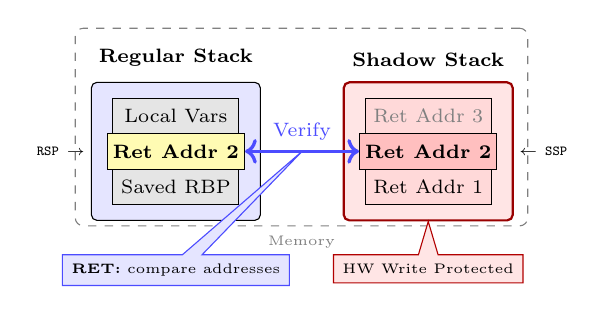
\begin{tikzpicture}[font=\scriptsize,
                stack title/.style={font=\scriptsize\bfseries},
                stack cell/.style={draw, minimum width=1.6cm, minimum height=0.45cm, anchor=north, inner sep=2pt},
                stack container/.style={draw, fill=#1, rounded corners=2pt}]

                % Regular Stack using matrix
                \matrix[matrix of nodes,
                    nodes={stack cell},
                    row sep=-\pgflinewidth,
                    column sep=0pt] (regstack) {
                    |[fill=gray!20]| Local Vars \\
                    |[fill=yellow!30, font=\scriptsize\bfseries]| Ret Addr 2 \\
                    |[fill=gray!20]| Saved RBP \\
                };
                \node[stack title, above=0.15cm of regstack] (regtitle) {Regular Stack};
                \begin{scope}[on background layer]
                    \node[stack container=blue!10, fit=(regstack), inner sep=2pt] {};
                \end{scope}

                % Shadow Stack using matrix (1.2cm = 0.8cm + 4mm)
                \matrix[matrix of nodes,
                    nodes={stack cell},
                    row sep=-\pgflinewidth,
                    right=1.2cm of regstack] (shadowstack) {
                    |[fill=red!15, text=gray]| Ret Addr 3 \\
                    |[fill=red!25, font=\scriptsize\bfseries]| Ret Addr 2 \\
                    |[fill=red!15]| Ret Addr 1 \\
                };
                \node[stack title, above=0.15cm of shadowstack] (sstitle) {Shadow Stack};
                \begin{scope}[on background layer]
                    \node[stack container=red!10, draw=red!60!black, thick,
                          fit=(shadowstack), inner sep=2pt] (sscontainer) {};
                \end{scope}

                % RSP pointer (pointing to Ret Addr 2)
                \node[font=\tiny\ttfamily, left=0.15cm of regstack-2-1.west] (rsp) {RSP $\rightarrow$};

                % SSP pointer (pointing to Ret Addr 2 in shadow stack)
                \node[font=\tiny\ttfamily, right=0.15cm of shadowstack-2-1.east] (ssp) {$\leftarrow$ SSP};

                % Memory region box (including titles)
                \begin{scope}[on background layer]
                    \node[draw=gray, dashed, rounded corners=3pt,
                          fit=(regtitle)(sstitle)(regstack)(shadowstack),
                          inner xsep=5pt, inner ysep=4pt,
                          label={[font=\tiny, gray]below:Memory}] (membox) {};
                \end{scope}

                % Stage 1: Only HW Write Protected callout
                \node[rectangle callout, draw=red!70!black, fill=red!10, font=\tiny,
                      callout absolute pointer={(sscontainer.south)},
                      below=0.5cm of shadowstack.south, anchor=north] {HW Write Protected};

                % Stage 2: Verify arrow and RET callout
                \visible<2->{
                    % Verify arrow between Ret Addr 2 entries
                    \draw[<->, very thick, blue!70] (regstack-2-1.east) -- (shadowstack-2-1.west)
                        node[midway, above, font=\scriptsize] {Verify};

                    % RET: verify callout below regular stack
                    \node[rectangle callout, draw=blue!70, fill=blue!10, font=\tiny,
                          callout absolute pointer={($(regstack-2-1.east)!0.5!(shadowstack-2-1.west)$)},
                          below=0.5cm of regstack.south, anchor=north] {\textbf{RET:} compare addresses};
                }
            \end{tikzpicture}
        \end{column}
    \end{columns}
\end{frame}
\begin{frame}{x86 Segmentation - The Original Security Model}
    \begin{columns}
        \begin{column}{0.5\textwidth}
            \textbf{Segmentation (Historical):}
            \begin{itemize}
                \item Original x86 protection mechanism
                \item Gates for controlled transitions
                \item Complex and rarely used today
            \end{itemize}
            
            \vspace{0.3cm}
            \textbf{Privilege Checking:}
            \begin{tcolorbox}[colback=yellow!20, boxsep=0pt]
                MAX(CPL, RPL) $\leq$ DPL
            \end{tcolorbox}
            \vspace{-2mm}
            \begin{itemize}
                \item \textbf{CPL}: Current Privilege Level
                \item \textbf{RPL}: Requested Privilege Level
                \item \textbf{DPL}: Descriptor Privilege Level
            \end{itemize}
        \end{column}
        \begin{column}{0.5\textwidth}
            \textbf{Gates (Obsolete):}
            \begin{itemize}
                \item Call Gates: Ring transitions
                \item Interrupt Gates: Hardware interrupts
                \item Trap Gates: Software interrupts
                \item Task Gates: Task switching
            \end{itemize}
            
            \vspace{-0.2cm}
            \begin{tcolorbox}[colback=red!10]
                \textbf{Reality Today:}
                \begin{itemize}
                    \item \textbf{Paging is the only protection}
                    \item Flat memory model (CS=DS=ES=SS)
                    \item Segments set to base=0, limit=4GB
                    \item Only Ring 0 and Ring 3 used
                \end{itemize}
            \end{tcolorbox}
        \end{column}
    \end{columns}
\end{frame}

\begin{frame}{Security Rings - x86 Architecture}
    \begin{columns}[T]
        \begin{column}{0.45\textwidth}
            \textbf{Modern Usage:}
            \begin{itemize}
                \item Ring 3: User applications
                \item Ring 1-2: Unused in practice
                \item Ring 0: Kernel (OS)
                \item Ring -1: Hypervisor\\
                      {\small (runs virtual machines)}
                \item Ring -2: SMM firmware\\
                      {\small (low-level hardware control)}
            \end{itemize}
        \end{column}
        \begin{column}{0.55\textwidth}
            \centering
            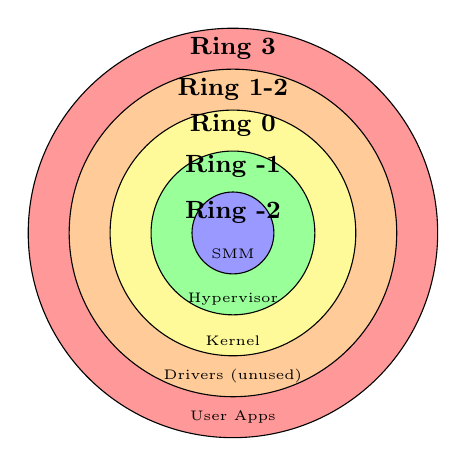
\begin{tikzpicture}[scale=0.65,
                ring num/.style={font=\small\bfseries},
                ring usage/.style={font=\tiny}]
                % Draw visible rings first
                \draw[fill=red!40] (0,0) circle (4cm);
                \draw[fill=orange!40] (0,0) circle (3.2cm);
                \draw[fill=yellow!40] (0,0) circle (2.4cm);

                % Standard rings labels - number at top, usage at bottom
                \node[ring num] at (0,3.6) {Ring 3};
                \node[ring usage] at (0,-3.6) {User Apps};

                \node[ring num] at (0,2.8) {Ring 1-2};
                \node[ring usage] at (0,-2.8) {Drivers (unused)};

                \node[ring num] at (0,2.1) {Ring 0};
                \node[ring usage] at (0,-2.1) {Kernel};

                % Inner rings (Ring -1 and Ring -2)
                \draw[fill=green!40] (0,0) circle (1.6cm);
                \node[ring num] at (0,1.3) {Ring -1};
                \node[ring usage] at (0,-1.3) {Hypervisor};

                \draw[fill=blue!40] (0,0) circle (0.8cm);
                \node[ring num] at (0,0.4) {Ring -2};
                \node[ring usage] at (0,-0.4) {SMM};
            \end{tikzpicture}
        \end{column}
    \end{columns}
\end{frame}

\begin{frame}{ARM TrustZone - Trusted Execution Environment (TEE)}
    \begin{center}
        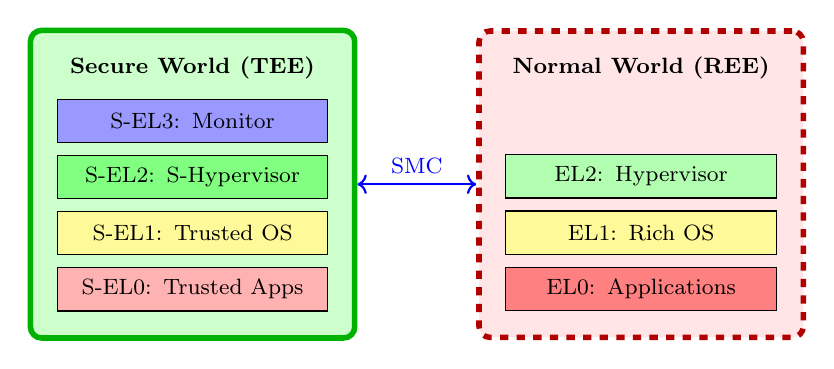
\begin{tikzpicture}[font=\footnotesize,
            level/.style={draw, text width=3.2cm, minimum height=0.55cm, align=center},
            empty/.style={draw=none, text width=3.2cm, minimum height=0.55cm}]

            % Secure World levels as matrix with named label
            \matrix[matrix of nodes, row sep=0.15cm, nodes={level},
                    label={[name=slabel, font=\footnotesize\bfseries]above:Secure World (TEE)}] (secure) {
                |[fill=blue!40]| S-EL3: Monitor \\
                |[fill=green!50]| S-EL2: S-Hypervisor \\
                |[fill=yellow!40]| S-EL1: Trusted OS \\
                |[fill=red!30]| S-EL0: Trusted Apps \\
            };

            % Secure World container using fit (includes label)
            \begin{scope}[on background layer]
                \node[rounded corners, fill=green!20, draw=green!70!black, line width=2pt,
                      fit=(slabel)(secure), inner sep=6pt] (scontainer) {};
            \end{scope}

            % Normal World levels as matrix with phantom top row
            \matrix[matrix of nodes, row sep=0.15cm, nodes={level},
                    right=2cm of secure,
                    label={[name=nlabel, font=\footnotesize\bfseries]above:Normal World (REE)}] (normal) {
                |[empty]| \\
                |[fill=green!30]| EL2: Hypervisor \\
                |[fill=yellow!40]| EL1: Rich OS \\
                |[fill=red!50]| EL0: Applications \\
            };

            % Normal World container using fit (includes label)
            \begin{scope}[on background layer]
                \node[rounded corners, fill=red!10, draw=red!70!black, line width=2pt, dashed,
                      fit=(nlabel)(normal), inner sep=6pt] (ncontainer) {};
            \end{scope}

            % SMC transition
            \draw[<->, thick, blue] (scontainer.east) -- (ncontainer.west) node[midway, above] {SMC};
        \end{tikzpicture}
    \end{center}

    \begin{columns}[T]
        \begin{column}{0.4\textwidth}
            \textbf{TEE Use Cases:}
            \begin{itemize}
                \item DRM content protection
                \item Mobile payments
                \item Biometric authentication
                \item Key management
            \end{itemize}
        \end{column}
        \begin{column}{0.6\textwidth}
            \textbf{TEE = Trusted Execution Environment}
            \begin{itemize}
                \item Isolated from Rich OS (REE)
                \item Secure boot chain
                \item Cryptographic operations
                \item Hardware root of trust
            \end{itemize}
        \end{column}
    \end{columns}
\end{frame}

\begin{frame}{Hardware Virtualization}
    \begin{columns}[T]
        \begin{column}{0.5\textwidth}
            \textbf{Virtualization:} Run multiple OSes on one machine
            \begin{itemize}
                \item Each VM thinks it has dedicated hardware
                \item Hypervisor multiplexes physical resources
            \end{itemize}

            \vspace{0.2cm}
            \textbf{Trap \& Emulate:}
            \begin{itemize}
                \item Guest runs normally until privileged op
                \item CPU traps to hypervisor (VM-Exit)
                \item Hypervisor emulates the operation
                \item Returns control to guest (VM-Entry)
            \end{itemize}

            \vspace{0.2cm}
            {\small \textit{Hardware: Intel VT-x, AMD-V, EPT/NPT for page tables}}
        \end{column}
        \begin{column}{0.5\textwidth}
            \centering
            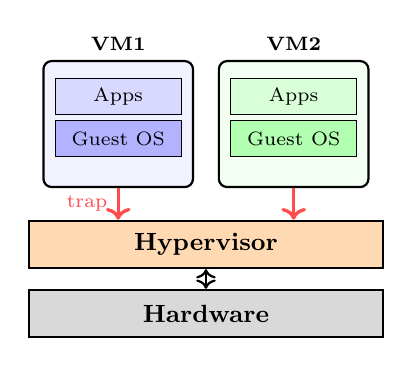
\begin{tikzpicture}[
                layer/.style={draw, thick, minimum width=4.5cm, minimum height=0.6cm, align=center, font=\small},
                vmbox/.style={draw, thick, minimum width=1.9cm, minimum height=1.6cm, rounded corners=3pt, fill=blue!5},
                vmlayer/.style={draw, minimum width=1.6cm, minimum height=0.45cm, align=center, font=\scriptsize}]

                % Hardware (bottom)
                \node[layer, fill=gray!30] (hw) {\textbf{Hardware}};

                % Hypervisor
                \node[layer, fill=orange!30, above=0.25cm of hw] (vmm) {\textbf{Hypervisor}};

                % VM boxes - increased spacing
                \node[vmbox, above left=0.4cm and 0.15cm of vmm.north, label={[font=\scriptsize\bfseries]above:VM1}] (vm1) {};
                \node[vmbox, fill=green!5, above right=0.4cm and 0.15cm of vmm.north, label={[font=\scriptsize\bfseries]above:VM2}] (vm2) {};

                % VM1 contents
                \node[vmlayer, fill=blue!15] at ([yshift=0.35cm]vm1.center) (app1) {Apps};
                \node[vmlayer, fill=blue!30, below=2pt of app1] (os1) {Guest OS};

                % VM2 contents
                \node[vmlayer, fill=green!15] at ([yshift=0.35cm]vm2.center) (app2) {Apps};
                \node[vmlayer, fill=green!30, below=2pt of app2] (os2) {Guest OS};

                % VM-Exit/Entry arrows
                \draw[->, very thick, red!70] (vm1.south) -- (vm1.south |- vmm.north)
                    node[midway, left, font=\scriptsize, text=red!70] {trap};
                \draw[->, very thick, red!70] (vm2.south) -- (vm2.south |- vmm.north);

                % Hardware access
                \draw[<->, thick] (vmm.south) -- (hw.north);
            \end{tikzpicture}

            \vspace{0.3cm}
            \textbf{Hardware Redirection (avoid exits):}
            \begin{itemize}
                \item EPT/NPT: Guest page tables
                \item Posted interrupts: Direct to guest
                \item VMCS shadowing: Nested VMs
            \end{itemize}
        \end{column}
    \end{columns}
\end{frame}

\begin{frame}{EPT/NPT - Nested Page Tables}
    \begin{columns}[T]
        \begin{column}{0.5\textwidth}
            \textbf{Problem:}
            \begin{itemize}
                \item Guest OS manages its own page tables
                \item Guest thinks it controls physical memory
                \item Hypervisor must translate guest physical $\rightarrow$ host physical
            \end{itemize}

            \vspace{0.2cm}
            \textbf{Solution: EPT/NPT}
            \begin{itemize}
                \item \textbf{EPT}: Intel's Extended Page Tables
                \item \textbf{NPT}: AMD's Nested Page Tables
                \item Hardware-accelerated 2D page walk
            \end{itemize}
        \end{column}
        \begin{column}{0.5\textwidth}
            \textbf{Address Translation:}
            \begin{enumerate}
                \item Guest Virtual $\rightarrow$ Guest Physical\\
                      {\small (guest page tables)}
                \item Guest Physical $\rightarrow$ Host Physical\\
                      {\small (EPT/NPT)}
            \end{enumerate}

            \vspace{0.3cm}
            \begin{tcolorbox}[colback=blue!10]
                \small
                \textbf{Key:} Every guest memory access (including page table walks) must go through EPT translation
            \end{tcolorbox}
        \end{column}
    \end{columns}
\end{frame}

\begin{frame}{2D Page Walk with EPT/NPT}
    \begin{columns}[T]
        \begin{column}{0.6\textwidth}
            \centering
            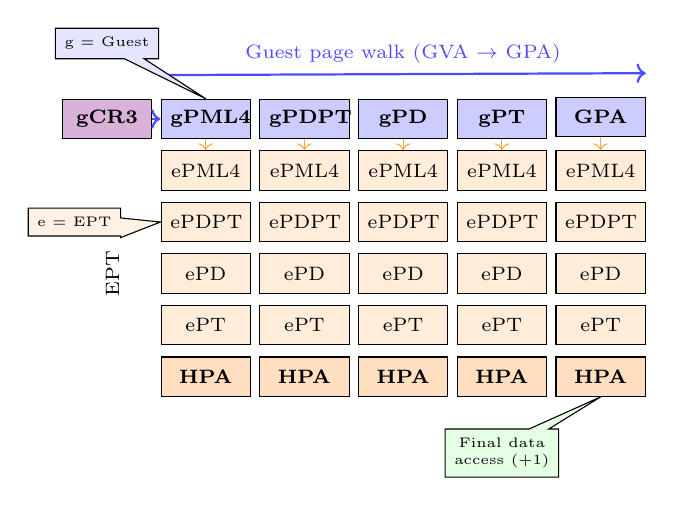
\begin{tikzpicture}
                \matrix[matrix of nodes,
                    ampersand replacement=\&,
                    nodes={minimum width=1.0cm, text width=0.9cm, minimum height=0.5cm, font=\scriptsize, align=center},
                    row 1/.style={nodes={fill=blue!20, draw, font=\scriptsize\bfseries}},
                    row 2/.style={nodes={fill=orange!15, draw}},
                    row 3/.style={nodes={fill=orange!15, draw}},
                    row 4/.style={nodes={fill=orange!15, draw}},
                    row 5/.style={nodes={fill=orange!15, draw}},
                    row 6/.style={nodes={fill=orange!25, draw, font=\scriptsize\bfseries}},
                    column 1/.style={nodes={draw=none, fill=none}},
                    row sep=4pt,
                    column sep=3pt] (m) {
                    |[draw, fill=violet!30]| gCR3 \& gPML4 \& gPDPT \& gPD \& gPT \& GPA \\
                    \& ePML4 \& ePML4 \& ePML4 \& ePML4 \& ePML4 \\
                    \& ePDPT \& ePDPT \& ePDPT \& ePDPT \& ePDPT \\
                    \& ePD \& ePD \& ePD \& ePD \& ePD \\
                    \& ePT \& ePT \& ePT \& ePT \& ePT \\
                    \& HPA \& HPA \& HPA \& HPA \& HPA \\
                };

                % Guest walk arrow (horizontal above matrix)
                \draw[->, thick, blue!70] (m-1-1.east) -- (m-1-2.west);
                \draw[->, thick, blue!70] ([yshift=0.3cm]m-1-2.north west) -- ([yshift=0.3cm]m-1-6.north east)
                    node[midway, above, font=\scriptsize] {Guest page walk (GVA $\rightarrow$ GPA)};

                % EPT walk label (vertical on left)
                \node[font=\scriptsize, rotate=90, anchor=south] at ([xshift=-0.4cm]m-4-2.west) {EPT};

                % Downward arrows for each column (skip column 1 which is CR3)
                \foreach \col in {2,3,4,5,6} {
                    \draw[->, thin, orange!70] (m-1-\col.south) -- (m-2-\col.north);
                }

                % Callouts (staged reveal)
                \visible<2->{
                    \node[rectangle callout, draw, fill=blue!10, font=\tiny,
                          callout absolute pointer={(m-1-2.north)},
                          above=5mm of m-1-1] {g = Guest};

                    \node[rectangle callout, draw, fill=orange!10, font=\tiny,
                          callout absolute pointer={(m-3-2.west)},
                          anchor=east] at ([xshift=-0.5cm]m-3-2.west) {e = EPT};
                }

                \visible<3->{
                    \node[rectangle callout, draw, fill=green!10, font=\tiny, align=center,
                          callout absolute pointer={(m-6-6.south)},
                          below=0.4cm of m-6-5] {Final data\\access (+1)};
                }
            \end{tikzpicture}
        \end{column}
        \begin{column}{0.4\textwidth}
            {\small Memory accesses (worst case):}

            \vspace{0.1cm}
            \begin{tcolorbox}[colback=blue!10, fontupper=\small, width=\textwidth-0.5cm]
                \textbf{Native:} 4 + 1 = \textbf{5}\\
                {\scriptsize 4 translation + 1 data}
            \end{tcolorbox}

            \vspace{0.1cm}
            \begin{tcolorbox}[colback=orange!15, fontupper=\small, width=\textwidth-0.5cm]
                \textbf{With EPT:} 24 + 1 = \textbf{25}\\
                {\scriptsize 24 translation + 1 data}
            \end{tcolorbox}

            \vspace{0.1cm}
            \textbf{Mitigations:}
            \begin{itemize}
                \item TLB caching
                \item Large pages
            \end{itemize}
        \end{column}
    \end{columns}
\end{frame}

\begin{frame}{IOMMU - Input/Output Memory Management Unit}
    \begin{columns}
        \begin{column}{0.55\textwidth}
            \textbf{What is IOMMU?}
            \begin{itemize}
                \item Hardware unit controlling device DMA
                \item Maps device addresses to physical memory
                \item Similar to MMU but for devices
            \end{itemize}

            \vspace{0.3cm}
            \textbf{Key Features:}
            \begin{itemize}
                \item \textbf{PASID:} Process Address Space ID
                \begin{itemize}
                    \item Like ASID but for devices
                    \item Allows device access to specific process memory
                \end{itemize}
                \item \textbf{Protection Granularity:} Page-level (4KB)
                \item \textbf{Interrupt Remapping:} Prevents interrupt injection
            \end{itemize}
        \end{column}
        \begin{column}{0.45\textwidth}
            \centering
            \begin{tikzpicture}[font=\footnotesize, scale=1.3, every node/.style={scale=1.3}]
                % Memory at top right
                \node[inner sep=0pt] (mem)
                    {\includegraphics[width=1cm]{figures/noun-ram-7483151.png}};
                \node[font=\tiny, above=1pt of mem] {Memory};

                % MMU as simple rectangle, left of Memory
                \node[draw, thick, fill=blue!20, minimum width=1.2cm, minimum height=0.6cm,
                      font=\scriptsize, left=0.4cm of mem] (mmu) {MMU};

                % CPU image left of MMU
                \node[inner sep=0pt, left=0.4cm of mmu] (cpu)
                    {\includegraphics[width=1cm]{figures/noun-cpu-8157304.png}};
                \node[font=\tiny, above=1pt of cpu] {CPU};

                % Wire CPU to MMU to Memory
                \draw[->, thick, blue] (cpu.east) -- (mmu.west);
                \draw[->, thick, blue] (mmu.east) -- (mem.west);

                % IOMMU as muxdemux - below MMU, with 3 bottom pins
                \node[muxdemux, muxdemux def={NB=3, Rh=1.5, Lh=1.5, w=3},
                      fill=yellow!30, thick, font=\small,
                      external pins width=0, below=0.8cm of mmu] (iommu) {IOMMU};

                % Wire from IOMMU top to Memory (with label on right)
                \draw[->, thick, green!60!black] (iommu.top) -- ++(0,0.15) -| (mem.south)
                    node[pos=0.75, right, font=\scriptsize] {Allowed};

                % Device images at bottom - spread out with explicit x offsets
                \node[inner sep=0pt, below=0.5cm of iommu.bpin 2] (nic)
                    {\includegraphics[width=0.8cm]{figures/noun-network-card-7443121.png}};
                \node[font=\tiny, below=1pt of nic] {NIC};

                \node[inner sep=0pt, left=0.8cm of nic] (usb)
                    {\includegraphics[width=0.8cm]{figures/noun-usb-8182582.png}};
                \node[font=\tiny, below=1pt of usb] {USB};

                \node[inner sep=0pt, right=0.8cm of nic] (gpu)
                    {\includegraphics[width=0.8cm]{figures/noun-graphics-card-1036913.png}};
                \node[font=\tiny, below=1pt of gpu] {GPU};

                % Device connections to IOMMU (DMA requests)
                \draw[->, thick, red] (usb.north) -- ++(0,0.15) -| (iommu.bpin 1);
                \draw[->, thick, red] (nic.north) -- (iommu.bpin 2);
                \draw[->, thick, red] (gpu.north) -- ++(0,0.15) -| (iommu.bpin 3);

                % Blocked indicator with X image
                \node[inner sep=0pt, right=0.6cm of iommu.right] (blocked)
                    {\includegraphics[width=0.5cm]{figures/noun-x-2222229.png}};
                \node[red, font=\scriptsize, below=1pt of blocked] {Blocked};

                % Show a blocked path attempt
                \draw[->, thick, red, dashed] (iommu.right) -- (blocked.west);
            \end{tikzpicture}
        \end{column}
    \end{columns}
\end{frame}
\begin{frame}{IOMMU - Attack Prevention}
    \begin{columns}
        \begin{column}{0.5\textwidth}
            \textbf{CPU-Initiated Attacks:}
            \begin{itemize}
                \item Compromised driver attempts DMA
                \item Kernel bug triggers bad DMA request
                \item IOMMU validates all translations
            \end{itemize}

            \vspace{0.5cm}
            \textbf{Device-Initiated Attacks:}
            \begin{itemize}
                \item Malicious firmware in peripherals
                \item Compromised network cards
                \item Rogue Thunderbolt devices
                \item USB devices with DMA capability
            \end{itemize}
        \end{column}
        \begin{column}{0.5\textwidth}
            \textbf{Attacks Prevented:}
            \begin{itemize}
                \item \textcolor{red}{DMA attacks} (BadUSB, Thunderstrike)
                \item \textcolor{red}{Malicious devices} reading memory
                \item \textcolor{red}{Driver bugs} corrupting memory
            \end{itemize}

            \vspace{0.5cm}
            \begin{tcolorbox}[colback=yellow!20]
                \textbf{Limitation:} Protection is page-granular (4KB). If two data structures share a page, device can access both!
            \end{tcolorbox}
        \end{column}
    \end{columns}
\end{frame}
% Management Engines and IOMMU
\begin{frame}{Intel Management Engine (ME)}
    \begin{columns}
        \begin{column}{0.5\textwidth}
            \textbf{What is Intel ME?}
            \begin{itemize}
                \item Separate processor on Intel chipsets
                \item Runs even when main CPU is off
                \item Full memory/network access (Ring -3)
                \item Cannot be disabled on modern systems
            \end{itemize}

            \vspace{0.2cm}
            \textbf{Legitimate Uses:}
            \begin{itemize}
                \item Remote management (AMT)
                \item Boot verification, DRM, anti-theft
            \end{itemize}

            \vspace{0.2cm}
            \textbf{Security Concerns:}
            \begin{itemize}
                \item Closed source firmware
                \item History of vulnerabilities
                \item Potential backdoor vector
            \end{itemize}
        \end{column}
        \begin{column}{0.5\textwidth}
            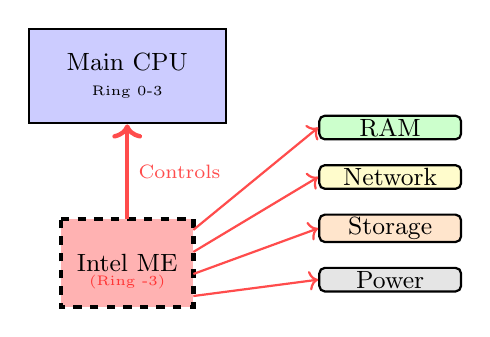
\begin{tikzpicture}[
                resource/.style={draw, thick, minimum width=1.8cm, minimum height=0.3cm,
                               align=center, font=\small, rounded corners=2pt, inner sep=1pt},
                cpu/.style={draw, thick, minimum width=2.5cm, minimum height=1.2cm,
                           fill=blue!20, align=center, font=\small},
                connection/.style={->, thick, red!70}]

                % Intel ME as muxdemux (center-left) - wider and shorter
                \node[muxdemux, muxdemux def={NL=1, NR=4, Rh=2, Lh=2, w=3},
                      fill=red!30, thick, dashed, font=\small, external pins width=0] (me)
                    {Intel ME};

                % Ring privilege level label (clearer)
                \node[font=\tiny, below=1pt of me.center, anchor=north, text=red!80]
                    {(Ring -3)};

                % Main CPU above ME
                \node[cpu, above=1.2cm of me.top] (cpu)
                    {Main CPU\\[-2pt]{\tiny Ring 0-3}};

                % Resources on the right side - RAM moved higher, others stacked below
                \node[resource, fill=green!20] (ram) at ([xshift=2.5cm,yshift=1.3cm]me.rpin 1) {RAM};
                \node[resource, fill=yellow!20, below=0.3cm of ram] (network) {Network};
                \node[resource, fill=orange!20, below=0.3cm of network] (storage) {Storage};
                \node[resource, fill=gray!20, below=0.3cm of storage] (power) {Power};

                % ME connections to resources
                \draw[connection] (me.rpin 1) -- (ram.west);
                \draw[connection] (me.rpin 2) -- (network.west);
                \draw[connection] (me.rpin 3) -- (storage.west);
                \draw[connection] (me.rpin 4) -- (power.west);

                % ME controls CPU
                \draw[connection, ultra thick] (me.top) -- (cpu.south)
                    node[midway, right, font=\scriptsize, text=red!70] {Controls};
            \end{tikzpicture}

            \begin{tcolorbox}[colback=yellow!20, fontupper=\scriptsize]
                \textbf{Similar:} AMD PSP, ARM TrustZone
            \end{tcolorbox}
        \end{column}
    \end{columns}
\end{frame}



% Subsection: Trusted Execution Environments
\subsection{Trusted Execution Environments}

\begin{frame}{Why Trusted Execution Environments (TEEs)?}
    \begin{columns}[T]
        \begin{column}{0.5\textwidth}
            \textbf{The Problem:}
            \begin{itemize}
                \item Cloud computing $\rightarrow$ running on untrusted infrastructure
                \item Cloud provider has physical access
                \item Hypervisor has full control over VMs
                \item Can read memory, modify code, inject malware
            \end{itemize}

            \vspace{0.3cm}
            \textbf{Trust Boundary Shift:}
            \begin{itemize}
                \item Traditional: Trust the cloud provider
                \item TEE: Trust only the hardware/CPU
                \item Provider is explicitly \textcolor{red}{untrusted}
            \end{itemize}
        \end{column}
        \begin{column}{0.5\textwidth}
            \textbf{Use Cases:}
            \begin{itemize}
                \item Confidential computing in public cloud
                \item Processing sensitive data (medical, financial)
                \item DRM / content protection
            \end{itemize}

            \vspace{-3mm}
            \begin{tcolorbox}[colback=blue!10, title={\small Goal}, boxsep=1pt]
                \textbf{Run code on someone else's hardware without them being able to:}%
                \begin{itemize}
                    \item Read your data
                    \item Modify your code
                    \item Tamper with execution
                \end{itemize}
                Even with physical access!
            \end{tcolorbox}

            \vspace{0.1cm}
            {\small \textit{VM-level (TDX/SEV) vs Process-level (SGX/TrustZone)}}
        \end{column}
    \end{columns}
\end{frame}

\begin{frame}{TEE Requirements - How Do We Achieve This?}
    \begin{columns}
        \begin{column}{0.5\textwidth}
            \textbf{1. Memory Encryption:}
            \begin{itemize}
                \item Encrypt all TEE memory
                \item Each TEE has unique encryption key
                \item Hardware encrypts/decrypts transparently
                \item Prevents physical memory dumps
            \end{itemize}

            \vspace{0.3cm}
            \textbf{2. Hardware-Enforced Isolation:}
            \begin{itemize}
                \item CPU enforces access control
                \item Hypervisor \textcolor{red}{cannot} access TEE memory
                \item DMA attacks blocked (IOMMU protection)
                \item Hardware prevents tampering
            \end{itemize}
        \end{column}
        \begin{column}{0.5\textwidth}
            \textbf{3. Remote Attestation:}
            \begin{itemize}
                \item Prove you're running in genuine TEE
                \item Relies on secure boot chain
                \item CPU signs measurement report
                \item Client verifies before sending secrets
            \end{itemize}

            \vspace{0.3cm}
            \textit{Relies on:}
            \begin{itemize}
                \item Secure boot (chain of trust)
                \item Hardware root of trust (TPM/fused keys)
                \item CPU manufacturer's PKI
            \end{itemize}
        \end{column}
    \end{columns}
\end{frame}

\begin{frame}{Remote Attestation Flow}
    \begin{columns}[T]
        \begin{column}{0.45\textwidth}
            \textbf{Attestation Steps:}
            \begin{enumerate}
                \item TEE measures code/data (hash)
                \item CPU signs measurement with private key
                \item Client verifies signature with CPU's public key
                \item If valid → client sends encrypted secrets
            \end{enumerate}

            \vspace{0.3cm}
            \textbf{Why It Works:}
            \begin{itemize}
                \item CPU private key burned in at manufacturing
                \item Cannot be extracted or forged
                \item Measurement reflects actual running code
            \end{itemize}
        \end{column}
        \begin{column}{0.55\textwidth}
            \centering
            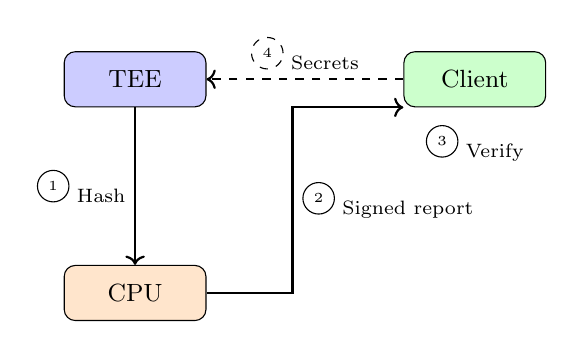
\begin{tikzpicture}[
                box/.style={draw, rounded corners, minimum width=1.8cm, minimum height=0.7cm, align=center, font=\small},
                arrow/.style={->, thick},
                num/.style={circle, draw, fill=white, font=\scriptsize, inner sep=1pt, minimum size=0.4cm}]

                % Entities
                \node[box, fill=blue!20] (tee) {TEE};
                \node[box, fill=green!20, right=2.5cm of tee] (client) {Client};
                \node[box, fill=orange!20, below=2cm of tee] (cpu) {CPU};

                % Arrows with circled numbers
                \draw[arrow] (tee) -- (cpu) node[midway, left, font=\scriptsize] {\tikz\node[num]{\tiny 1}; Hash};
                \draw[arrow] (cpu) -- ++(2cm,0) |- (client.south west)
                    node[pos=0.25, right, font=\scriptsize] {\tikz\node[num]{\tiny 2}; Signed report};
                \node[font=\scriptsize, below=0.1cm of client] {\tikz\node[num]{\tiny 3}; Verify};
                \draw[arrow, dashed] (client) -- (tee) node[midway, above, font=\scriptsize] {\tikz\node[num]{\tiny 4}; Secrets};
            \end{tikzpicture}

            \vspace{0.3cm}
            \begin{tcolorbox}[colback=green!10, fontupper=\small]
                \textbf{Result:} Client is confident code is running in genuine TEE, unmodified
            \end{tcolorbox}
        \end{column}
    \end{columns}
\end{frame}

\begin{frame}{TEE Memory Protection Approaches (1/2)}
    \begin{columns}[T]
        \begin{column}{0.5\textwidth}
            \textbf{1. Access Control Based:}
            \begin{itemize}
                \item CPU enforces access restrictions
                \item Hypervisor/OS \textcolor{red}{blocked} from accessing TEE memory
                \item Page table attributes control access
                \item Fast (no encryption overhead)
                \item \textbf{Example:} SGX (EPCM), TrustZone (NS bit)
                \item \textcolor{red}{\textbf{Limitation:}} Physical attacks (cold boot, bus snooping)
            \end{itemize}
        \end{column}
        \begin{column}{0.5\textwidth}
            \textbf{2. Encryption Based:}
            \begin{itemize}
                \item Memory encrypted in DRAM
                \item Each TEE has unique key
                \item Hardware encrypts/decrypts on memory bus
                \item Protects against physical attacks
                \item \textbf{Example:} AMD SEV, Intel MKTME
            \end{itemize}
        \end{column}
    \end{columns}
\end{frame}

\begin{frame}{TEE Memory Protection Approaches (2/2)}
    \begin{columns}[T]
        \begin{column}{0.5\textwidth}
            \textbf{3. Hybrid Approaches:}

            \vspace{0.2cm}
            Combine both for defense in depth:
            \begin{itemize}
                \item Access control prevents software attacks
                \item Encryption prevents physical attacks
                \item \textbf{Example:} SEV-SNP (RMP), TDX (SEPT)
            \end{itemize}
        \end{column}
        \begin{column}{0.5\textwidth}
            \begin{tcolorbox}[colback=blue!10, title={\small Trade-offs}]
                \textbf{Access Control Only:}
                \begin{itemize}
                    \item[\checkmark] Fast, no encryption overhead
                    \item[$\times$] Physical attacks possible
                \end{itemize}

                \textbf{Encryption Only:}
                \begin{itemize}
                    \item[\checkmark] Protects against physical attacks
                    \item[$\times$] Performance overhead (5-15\%)
                \end{itemize}

                \textbf{Hybrid:}
                \begin{itemize}
                    \item[\checkmark] Defense in depth
                    \item[$\times$] Complexity + overhead
                \end{itemize}
            \end{tcolorbox}
        \end{column}
    \end{columns}
\end{frame}

\begin{frame}{Memory Integrity: Reverse Map Table (RMP)}
    \begin{columns}[T]
        \vspace{-5mm}
        \begin{column}{0.55\textwidth}
            \textbf{Problem:} Hypervisor controls page tables
            \begin{itemize}
                \item Can remap guest physical → host physical
                \item Could redirect VM memory to attacker pages
            \end{itemize}

            %\vspace{0.1cm}
            \textbf{Solution: Reverse Map Table (RMP)}
            \begin{itemize}
                \item One entry per physical page in system
                \item Tracks owner (which VM or hypervisor)
                \item Hardware checks RMP on \textbf{every} access
            \end{itemize}

            %\vspace{0.1cm}
            \textbf{Key Properties:} {\small (AMD SEV-SNP)}
            \begin{itemize}
                \item Each physical page has exactly one owner
                \item Hypervisor cannot access VM-owned pages
            \end{itemize}
        \end{column}
        \begin{column}{0.45\textwidth}
            \centering
            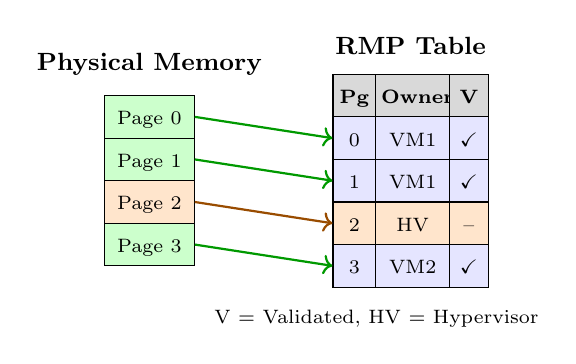
\begin{tikzpicture}[arrow/.style={->, thick}]
                % Physical Memory matrix
                \matrix[matrix of nodes,
                    ampersand replacement=\&,
                    label={[font=\small\bfseries]above:Physical Memory},
                    nodes={draw, text width=1cm, text height=0.3cm, text depth=0.1cm,
                           align=center, inner sep=2pt, font=\scriptsize, fill=green!20},
                    row sep=-\pgflinewidth] (mem) {
                    Page 0 \\
                    Page 1 \\
                    |[fill=orange!20]| Page 2 \\
                    Page 3 \\
                };

                % RMP Table matrix - positioned relative to mem
                \matrix[matrix of nodes,
                    ampersand replacement=\&,
                    right=1.5cm of mem,
                    label={[font=\small\bfseries]above:RMP Table},
                    nodes={draw, text height=0.3cm, text depth=0.1cm,
                           align=center, inner sep=2pt, font=\scriptsize, fill=blue!10},
                    column 1/.style={nodes={text width=0.4cm}},
                    column 2/.style={nodes={text width=0.8cm}},
                    column 3/.style={nodes={text width=0.35cm}},
                    row sep=-\pgflinewidth,
                    column sep=-\pgflinewidth,
                    row 1/.style={nodes={fill=gray!30, font=\scriptsize\bfseries}}] (rmp) {
                    Pg \& Owner \& V \\
                    0 \& VM1 \& \checkmark \\
                    1 \& VM1 \& \checkmark \\
                    |[fill=orange!20]| 2 \& |[fill=orange!20]| HV \& |[fill=orange!20]| -- \\
                    3 \& VM2 \& \checkmark \\
                };

                % Arrows between matrices (mem rows 1-4, rmp rows 2-5 since row 1 is header)
                \draw[arrow, green!60!black] (mem-1-1.east) -- (rmp-2-1.west);
                \draw[arrow, green!60!black] (mem-2-1.east) -- (rmp-3-1.west);
                \draw[arrow, orange!60!black] (mem-3-1.east) -- (rmp-4-1.west);
                \draw[arrow, green!60!black] (mem-4-1.east) -- (rmp-5-1.west);

                % Legend
                \node[font=\scriptsize, below=0.3cm of mem.south east, anchor=north west] {V = Validated, HV = Hypervisor};
            \end{tikzpicture}

            \vspace{0.2cm}
            \begin{tcolorbox}[colback=yellow!10, fontupper=\scriptsize]
                \textbf{Note:} Prevents remapping attacks but not full replay protection (no Merkle tree)
            \end{tcolorbox}
        \end{column}
    \end{columns}
\end{frame}

\begin{frame}{Secure VMs vs Secure Enclaves}
    \begin{columns}[T]
        \begin{column}{0.5\textwidth}
            \textbf{Secure Enclaves (Process-Level):}
            \begin{itemize}
                \item Isolate parts of an application
                \item Trust boundary \textit{within} a VM/OS
                \item Small trusted computing base (TCB)
                \item Application explicitly uses enclave
            \end{itemize}

            \vspace{0.2cm}
            \textbf{Threat Model:}
            \begin{itemize}
                \item Untrusted OS/kernel and applications
                \item Privileged software is adversary
            \end{itemize}

            \vspace{0.2cm}
            \textbf{Examples:}
            \begin{itemize}
                \item \textbf{Intel SGX}: x86 enclave instructions
                \item \textbf{ARM TrustZone}: Secure/Normal worlds
            \end{itemize}

            \vspace{0.2cm}
            \textbf{Use Cases:}
            \begin{itemize}
                \item Protect cryptographic keys
                \item Secure password verification
                \item DRM (Digital Rights Management)
            \end{itemize}
        \end{column}
        \begin{column}{0.5\textwidth}
            \textbf{Secure VMs (VM-Level):}
            \begin{itemize}
                \item Isolate entire virtual machines
                \item Trust boundary at hypervisor level
                \item Large TCB (entire VM)
                \item Transparent to guest OS
            \end{itemize}

            \vspace{0.2cm}
            \textbf{Threat Model:}
            \begin{itemize}
                \item Untrusted hypervisor/cloud provider
                \item Physical access attacks
            \end{itemize}

            \vspace{0.2cm}
            \textbf{Examples:}
            \begin{itemize}
                \item \textbf{Intel TDX}: Trust Domain Extensions
                \item \textbf{AMD SEV-SNP}: Secure Nested Paging
            \end{itemize}

            \vspace{0.2cm}
            \textbf{Use Cases:}
            \begin{itemize}
                \item Confidential computing in public cloud
                \item Lift-and-shift existing workloads
                \item Multi-tenant isolation
            \end{itemize}

            \vspace{0.2cm}
            \begin{tcolorbox}[colback=green!10]
                {\scriptsize \textbf{Key Difference:}\\
                Enclaves require application changes.\\
                Secure VMs work with unmodified OS.}
            \end{tcolorbox}
        \end{column}
    \end{columns}
\end{frame}


\begin{frame}[fragile]{Merkle Trees for Memory Freshness}
    \begin{columns}
        \begin{column}{0.5\textwidth}
            \textbf{The Replay Problem:}
            \begin{itemize}
                \item Encryption prevents reading
                \item But not replay attacks
                \item Attacker saves old ciphertext
                \item Replays it later
            \end{itemize}

            \vspace{0.2cm}
            \textbf{Merkle Tree Solution:} {\small (Intel SGX)}
            \begin{itemize}
                \item Tree of cryptographic hashes
                \item Root stored in secure on-chip memory
                \item Each node hashes its children
                \item Detects any modification/replay
            \end{itemize}

            %\textbf{Intel SGX Implementation:}
            %\begin{itemize}
            %    \item 8-ary tree (8 children per node)
            %    \item Counters at leaf level
            %    \item MAC for each cache line
            %    \item Root in on-chip SRAM
            %\end{itemize}
        \end{column}
        \begin{column}{0.5\textwidth}
            \centering
            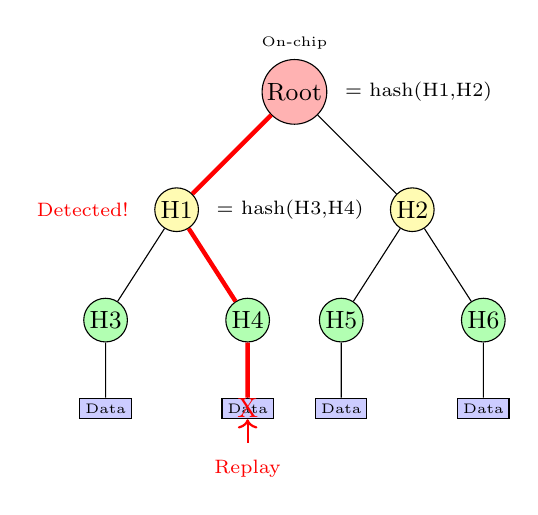
\begin{tikzpicture}[scale=0.75,
                level dist/.store in=\leveldist, level dist=1cm,
                sibling dist/.store in=\siblingdist, sibling dist=1cm,
                hashnode/.style={draw, circle, inner sep=1pt, font=\small}]
                % Root
                \node[hashnode, fill=red!30] (root) {Root};
                \node[above=0mm of root] {\tiny On-chip};
                \node[right=1mm of root, font=\scriptsize] {= hash(H1,H2)};

                % Level 1 - below root
                \node[hashnode, fill=yellow!30, below left=\leveldist and \siblingdist of root] (n1) {H1};
                \node[right=1mm of n1, font=\scriptsize] {= hash(H3,H4)};
                \node[hashnode, fill=yellow!30, below right=\leveldist and \siblingdist of root] (n2) {H2};

                % Level 2 - below level 1
                \node[hashnode, fill=green!30, below left=\leveldist and 0.5cm of n1] (n3) {H3};
                \node[hashnode, fill=green!30, below right=\leveldist and 0.5cm of n1] (n4) {H4};
                \node[hashnode, fill=green!30, below left=\leveldist and 0.5cm of n2] (n5) {H5};
                \node[hashnode, fill=green!30, below right=\leveldist and 0.5cm of n2] (n6) {H6};

                % Data blocks - below level 2 (one per H node for compactness)
                \node[draw,fill=blue!20, inner sep=2pt, below=0.7cm of n3] (d1) {\tiny Data};
                \node[draw,fill=blue!20, inner sep=2pt, below=0.7cm of n4] (d3) {\tiny Data};
                \node[draw,fill=blue!20, inner sep=2pt, below=0.7cm of n5] (d4) {\tiny Data};
                \node[draw,fill=blue!20, inner sep=2pt, below=0.7cm of n6] (d6) {\tiny Data};

                % Edges
                \draw[-] (root) -- (n1);
                \draw[-] (root) -- (n2);
                \draw[-] (n1) -- (n3);
                \draw[-] (n1) -- (n4);
                \draw[-] (n2) -- (n5);
                \draw[-] (n2) -- (n6);
                \draw[-] (n3) -- (d1);
                \draw[-] (n4) -- (d3);
                \draw[-] (n5) -- (d4);
                \draw[-] (n6) -- (d6);

                % Attack
                \node[red] at (d3) {X};
                \draw[->,thick,red] ([yshift=-0.4cm]d3.south) -- (d3.south);
                \node[red, font=\scriptsize, below=0.4cm of d3] {Replay};

                % Detection path
                \draw[ultra thick,red] (d3) -- (n4);
                \draw[ultra thick,red] (n4) -- (n1);
                \draw[ultra thick,red] (n1) -- (root);
                \node[red, font=\scriptsize, left=2mm of n1] {Detected!};
            \end{tikzpicture}
        \end{column}
    \end{columns}
\end{frame}

\begin{frame}{MKTME (Multi-Key Total Memory Encryption)}
    \begin{columns}
        \begin{column}{0.5\textwidth}
            \textbf{Features:}
            \begin{itemize}
                \item Multiple encryption keys
                \item Per-VM/container isolation
                \item KeyID in physical address bits
                \item AES-XTS encryption
            \end{itemize}
            
            \vspace{0.3cm}
            \textbf{Key Management:}
            \begin{itemize}
                \item Up to 15 keys (4-bit KeyID)
                \item Software-managed keys
                \item PCONFIG instruction
                \item Key rotation support
            \end{itemize}
        \end{column}
        \begin{column}{0.5\textwidth}
            \begin{tikzpicture}[scale=0.6, font=\small,
                addr field/.style={draw, minimum height=0.8cm, anchor=west},
                vm box/.style={draw, minimum width=2cm, minimum height=1.6cm, align=center}]

                % Physical address bar
                \node[addr field, fill=red!30, minimum width=1.2cm] (keyid) at (0,4) {};
                \node at (keyid.center) {KeyID};
                \node[addr field, fill=blue!30, minimum width=5.2cm, right=0pt of keyid] (paddr) {};
                \node at (paddr.center) {Physical Address};

                % Memory regions
                \node[vm box, fill=green!30] (vm1) at (1,1) {VM1\\{\scriptsize Encrypted}\\[-1pt]\includegraphics[height=0.25cm]{figures/noun-key-8095348.png}};
                \node[vm box, fill=blue!30, right=0.4cm of vm1] (vm2) {VM2\\{\scriptsize Encrypted}\\[-1pt]\includegraphics[height=0.25cm]{figures/noun-key-8095348.png}};
                \node[vm box, fill=yellow!30, right=0.4cm of vm2] (vm3) {VM3\\{\scriptsize Encrypted}\\[-1pt]\includegraphics[height=0.25cm]{figures/noun-key-8095348.png}};

                % Encryption engine
                \draw[thick,<->] (vm2.north) -- ++(0,1) node[right, midway] {AES-XTS};
            \end{tikzpicture}
            
            \vspace{0.3cm}
            \textbf{Use Cases:}
            \begin{itemize}
                \item Cloud multi-tenancy
                \item Container isolation
                \item Key-based memory domains
            \end{itemize}
        \end{column}
    \end{columns}
\end{frame}

% Section 5: Boot Security
\section{Boot Security}

\begin{frame}{Secure Boot - Chain of Trust}
    \begin{columns}[T]
        \begin{column}{0.6\textwidth}
            \textbf{Chain of Trust:}
            \begin{itemize}
                \item Each stage verifies the next before executing
                \item Hardware root of trust anchors the chain
                \item UEFI Secure Boot checks cryptographic signatures
                \item Blocks execution if signature invalid
            \end{itemize}

            \vspace{0.3cm}
            \textbf{Key Components:}
            \begin{itemize}
                \item \textbf{Root of Trust:} Immutable hardware anchor
                \item \textbf{UEFI Firmware:} First mutable code, verifies bootloader
                \item \textbf{Bootloader:} Verifies OS kernel signature
                \item \textbf{Kernel:} Enforces module signing
            \end{itemize}

            \vspace{0.3cm}
            \begin{tcolorbox}[colback=green!10, fontupper=\small]
                \textbf{Goal:} Prevent unauthorized code from running at boot time
            \end{tcolorbox}
        \end{column}
        \begin{column}{0.4\textwidth}
            \centering
            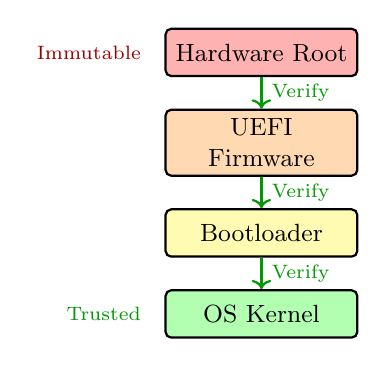
\begin{tikzpicture}[
                chainlink/.style={draw, thick, text width=2.2cm, minimum height=0.6cm,
                                 align=center, font=\small, rounded corners=2pt},
                verify/.style={->, thick, green!60!black}]

                % Boot Chain
                \node[chainlink, fill=red!30] (hw) {Hardware Root};
                \node[chainlink, fill=orange!30, below=0.4cm of hw] (uefi) {UEFI Firmware};
                \node[chainlink, fill=yellow!30, below=0.4cm of uefi] (bootloader) {Bootloader};
                \node[chainlink, fill=green!30, below=0.4cm of bootloader] (kernel) {OS Kernel};

                % Verification arrows (green)
                \draw[verify] (hw.south) -- (uefi.north)
                    node[midway, right, font=\scriptsize] {Verify};
                \draw[verify] (uefi.south) -- (bootloader.north)
                    node[midway, right, font=\scriptsize] {Verify};
                \draw[verify] (bootloader.south) -- (kernel.north)
                    node[midway, right, font=\scriptsize] {Verify};

                % Labels
                \node[font=\scriptsize, text=red!60!black, left=5pt of hw] {Immutable};
                \node[font=\scriptsize, text=green!60!black, left=5pt of kernel] {Trusted};
            \end{tikzpicture}

            \vspace{0.3cm}
            \begin{tcolorbox}[colback=blue!10, fontupper=\scriptsize]
                \textbf{Verification:} Each stage checks signature of next\\[1pt]
                \textbf{On Failure:} Boot halts -- unauthorized code blocked
            \end{tcolorbox}
        \end{column}
    \end{columns}
\end{frame}

\begin{frame}{Measured Boot with TPM}
    \begin{columns}[T]
        \begin{column}{0.6\textwidth}
            \textbf{Measured Boot:}
            \begin{itemize}
                \item Records what ran (doesn't block!)
                \item TPM stores hashes in PCRs
                \item Complements Secure Boot verification
            \end{itemize}

            \vspace{0.2cm}
            \textbf{PCR Extend Operation:}
            \begin{tcolorbox}[colback=gray!10]
                \small
                \texttt{PCR[i] = SHA256(PCR[i] \tikzmarknode{concatop}{||} data)}
            \end{tcolorbox}
            \begin{tikzpicture}[remember picture, overlay]
                \node[rectangle callout, draw, fill=yellow!20, font=\tiny,
                      callout absolute pointer={(concatop.north)},
                      above=0.15cm of concatop]
                      {concatenation};
            \end{tikzpicture}
            {\small Cannot directly overwrite -- only extend!}

            \vspace{0.2cm}
            \textbf{Remote Attestation:}
            \begin{itemize}
                \item Prove system state to remote party
                \item TPM signs PCR values with attestation key
                \item Enables conditional access/secrets
            \end{itemize}

            \vspace{0.2cm}
            {\small \textbf{IMA:} Runtime measurements extend to applications (PCR10)}
        \end{column}
        \begin{column}{0.4\textwidth}
            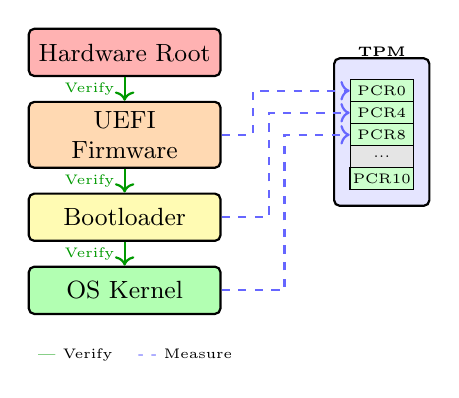
\begin{tikzpicture}[
                chainlink/.style={draw, thick, text width=2.2cm, minimum height=0.6cm,
                                 align=center, font=\small, rounded corners=2pt},
                verify/.style={->, thick, green!60!black},
                measure/.style={->, thick, blue!60, dashed}]

                % Boot Chain - left side
                \node[chainlink, fill=red!30] (hw) {Hardware Root};
                \node[chainlink, fill=orange!30, below=0.3cm of hw] (uefi) {UEFI Firmware};
                \node[chainlink, fill=yellow!30, below=0.3cm of uefi] (bootloader) {Bootloader};
                \node[chainlink, fill=green!30, below=0.3cm of bootloader] (kernel) {OS Kernel};

                % TPM with PCR matrix - right side
                \matrix[matrix of nodes,
                    nodes={draw, minimum width=0.8cm, minimum height=0.28cm,
                           font=\tiny, fill=green!20, inner sep=1pt},
                    row sep=-\pgflinewidth,
                    right=1.5cm of uefi] (pcrs) {
                    PCR0 \\
                    PCR4 \\
                    PCR8 \\
                    |[fill=gray!20]| ... \\
                    PCR10 \\
                };

                % TPM container around PCRs
                \node[font=\tiny\bfseries, above=1pt of pcrs] {TPM};
                \begin{scope}[on background layer]
                    \node[draw, thick, fill=blue!10, rounded corners=2pt,
                          fit={(pcrs) ([yshift=2pt]pcrs.north)}, inner sep=2pt] (tpm) {};
                \end{scope}

                % Verification arrows (green)
                \draw[verify] (hw.south) -- (uefi.north)
                    node[midway, left, font=\tiny] {Verify};
                \draw[verify] (uefi.south) -- (bootloader.north)
                    node[midway, left, font=\tiny] {Verify};
                \draw[verify] (bootloader.south) -- (kernel.north)
                    node[midway, left, font=\tiny] {Verify};

                % TPM measurement arrows (blue dashed) - smallest x for top PCR
                \draw[measure] (uefi.east) -- ++(0.4cm,0) |- (pcrs-1-1.west);
                \draw[measure] (bootloader.east) -- ++(0.6cm,0) |- (pcrs-2-1.west);
                \draw[measure] (kernel.east) -- ++(0.8cm,0) |- (pcrs-3-1.west);

                % Legend
                \node[font=\tiny, below=0.3cm of kernel.south west, anchor=north west] {
                    \textcolor{green!60!black}{---} Verify \quad
                    \textcolor{blue!60}{- -} Measure};
            \end{tikzpicture}

            \vspace{-0.8cm}
            \begin{tcolorbox}[colback=blue!10, fontupper=\scriptsize]
                \textbf{Key Difference:} Secure Boot \textit{blocks} unauthorized code;\\
                Measured Boot \textit{records} what ran for later attestation
            \end{tcolorbox}
        \end{column}
    \end{columns}
\end{frame}

% Section 6: Summary
\section{Summary}


\begin{frame}{Summary}
    \begin{itemize}
        \item \textbf{Defense in Depth:} Multiple layers of security mechanisms
        \vspace{0.3cm}
        \item \textbf{Hardware Acceleration:} Critical security features need hardware support for performance
        \vspace{0.3cm}
        \item \textbf{Trust Boundaries:} Clear separation between trusted and untrusted components
        \vspace{0.3cm}
        \item \textbf{Attestation:} Cryptographic proof of system state and configuration
        \vspace{0.3cm}
        \item \textbf{Memory Protection:} Tags, authentication, and encryption for memory safety
        \vspace{0.3cm}
        \item \textbf{Control Flow:} Hardware enforcement of valid program execution paths
    \end{itemize}
\end{frame}

\appendix
\begin{frame}
    \centering
    \Huge Backup
\end{frame}
\begin{frame}{Modern ROP Mitigations Summary}
    \begin{center}
        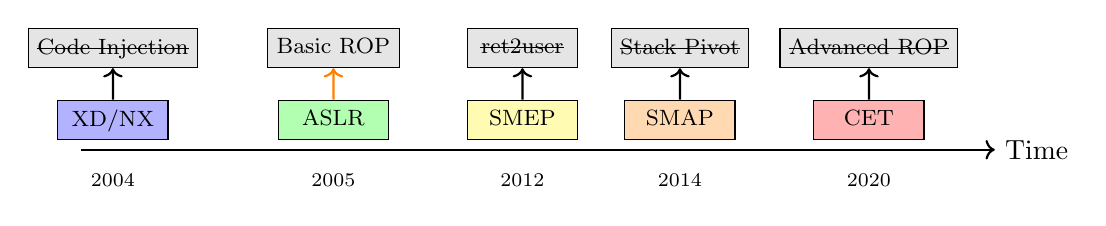
\begin{tikzpicture}[scale=0.8,
            year/.style={font=\scriptsize, text depth=0.25ex},
            defense/.style={draw, minimum width=1.4cm, minimum height=0.5cm, font=\footnotesize, text depth=0.25ex},
            attack/.style={draw, fill=gray!20, minimum width=1.4cm, minimum height=0.5cm, font=\footnotesize, text depth=0.25ex},
            mitigates/.style={->, thick},
            crossout/.style={thick, red}]

            % Timeline arrow - extended to avoid overlap with 2020
            \draw[thick,->] (-1.5,0) -- (13,0) node[right] {Time};

            % Year markers below the timeline
            \node[year] (y2004) at (-1,-0.5) {2004};
            \node[year] (y2005) at (2.5,-0.5) {2005};
            \node[year] (y2012) at (5.5,-0.5) {2012};
            \node[year] (y2014) at (8,-0.5) {2014};
            \node[year] (y2020) at (11,-0.5) {2020};

            % Defense nodes above timeline, aligned with years
            \node[defense, fill=blue!30, above=0.3cm of y2004] (nx) {XD/NX};
            \node[defense, fill=green!30, above=0.3cm of y2005] (aslr) {ASLR};
            \node[defense, fill=yellow!30, above=0.3cm of y2012] (smep) {SMEP};
            \node[defense, fill=orange!30, above=0.3cm of y2014] (smap) {SMAP};
            \node[defense, fill=red!30, above=0.3cm of y2020] (cet) {CET};

            % Attack nodes above defenses - close to the mechanism that stops them
            \node[attack, above=0.4cm of nx] (inject) {\sout{Code Injection}};
            \draw[mitigates] (nx) -- (inject);

            \node[attack, above=0.4cm of aslr] (rop) {Basic ROP};
            \draw[mitigates, orange] (aslr) -- (rop);

            \node[attack, above=0.4cm of smep] (ret2user) {\sout{ret2user}};
            \draw[mitigates] (smep) -- (ret2user);

            \node[attack, above=0.4cm of smap] (pivot) {\sout{Stack Pivot}};
            \draw[mitigates] (smap) -- (pivot);

            \node[attack, above=0.4cm of cet] (advanced) {\sout{Advanced ROP}};
            \draw[mitigates] (cet) -- (advanced);
        \end{tikzpicture}
    \end{center}
    
    \vspace{0.5cm}
    \begin{columns}
        \begin{column}{0.33\textwidth}
            \textbf{User Space:}
            \begin{itemize}
                \item XD/NX bit
                \item ASLR
                \item Stack Canaries
                \item CFI/CET
                \item Shadow Stack
            \end{itemize}
        \end{column}
        \begin{column}{0.33\textwidth}
            \textbf{Kernel Space:}
            \begin{itemize}
                \item SMEP (HW)
                \item SMAP (HW)
                \item KASLR (SW)
                \item KPTI* (SW)
                \item FineIBT (HW+SW)
            \end{itemize}
        \end{column}
        \begin{column}{0.33\textwidth}
            \textbf{Hardware:}
            \begin{itemize}
                \item Intel CET
                \item ARM PAC/BTI
                \item ARM MTE
                \item Control-flow integrity
            \end{itemize}
        \end{column}
    \end{columns}
    
    \vspace{0.2cm}
    \small *KPTI: Kernel Page Table Isolation - software mitigation for Meltdown
\end{frame}
\begin{frame}{Performance Impact of Security Features}
    \begin{center}
        \begin{tabular}{|l|c|c|l|}
            \hline
            \textbf{Feature} & \textbf{Type} & \textbf{Impact} & \textbf{Overhead} \\
            \hline
            \hline
            XD/NX Bit & HW & \cellcolor{green!30}Low & Page table bit check \\
            \hline
            SMEP & HW & \cellcolor{green!30}Low & Permission check \\
            \hline
            SMAP & HW & \cellcolor{green!30}Low & AC flag check \\
            \hline
            Stack Canaries & SW & \cellcolor{green!30}Low & Function epilogue check \\
            \hline
            ASLR & SW & \cellcolor{green!30}Low & One-time randomization \\
            \hline
            CET (Shadow Stack) & HW & \cellcolor{yellow!30}Medium & Parallel stack ops \\
            \hline
            PAC (ARM) & HW & \cellcolor{yellow!30}Medium & Crypto ops per call \\
            \hline
            BTI (ARM) & HW & \cellcolor{yellow!30}Medium & Branch checks \\
            \hline
            KASLR & SW & \cellcolor{yellow!30}Medium & Kernel relocation \\
            \hline
            KPTI* & SW & \cellcolor{orange!30}High & Page table switches \\
            \hline
            Full CFI** & SW & \cellcolor{orange!30}High & Type checks everywhere \\
            \hline
            FineIBT & HW+SW & \cellcolor{yellow!30}Medium & Hash + branch checks \\
            \hline
        \end{tabular}
    \end{center}
    
    \vspace{0.3cm}
    \begin{columns}
        \begin{column}{0.5\textwidth}
            \small
            *Software mitigation for Meltdown\\
            **Software-only implementation
        \end{column}
        \begin{column}{0.5\textwidth}
            \begin{tcolorbox}[colback=yellow!10]
                \small
                \textbf{Impact Categories:}
                \begin{itemize}
                    \item \textcolor{green!70!black}{Low}: $<$5\%
                    \item \textcolor{yellow!70!black}{Medium}: 5-15\%
                    \item \textcolor{orange!70!black}{High}: $>$15\%
                \end{itemize}
            \end{tcolorbox}
        \end{column}
    \end{columns}
\end{frame}
\begin{frame}{Hardware Security Evolution}
    \begin{center}
    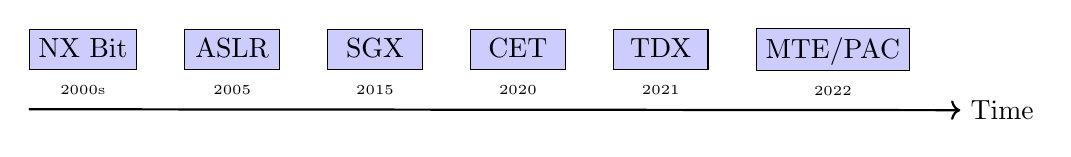
\begin{tikzpicture}[scale=0.8,
            timeline label/.style={font=\tiny, text depth=0.25ex},
            feature/.style={draw, fill=blue!20, minimum width=1.2cm, minimum height=0.5cm, text depth=0.25ex}]

            % Security features with consistent style
            \node[feature] (nx) at (1,0) {NX Bit};
            \node[timeline label, below=2pt of nx] (year-nx) {2000s};

            \node[feature, right=0.6cm of nx] (aslr) {ASLR};
            \node[timeline label, below=2pt of aslr] {2005};

            \node[feature, right=0.6cm of aslr] (sgx) {SGX};
            \node[timeline label, below=2pt of sgx] {2015};

            \node[feature, right=0.6cm of sgx] (cet) {CET};
            \node[timeline label, below=2pt of cet] {2020};

            \node[feature, right=0.6cm of cet] (tdx) {TDX};
            \node[timeline label, below=2pt of tdx] {2021};

            \node[feature, right=0.6cm of tdx] (mte) {MTE/PAC};
            \node[timeline label, below=2pt of mte] (year-mte) {2022};

            % Timeline arrow (positioned relative to nodes)
            \draw[thick,->] ([yshift=-1pt]nx.west |- year-nx.south) -- ([yshift=-1pt, xshift=0.8cm]mte.east |- year-mte.south) node[right] {Time};
        \end{tikzpicture}
    \end{center}

    \vspace{0.3cm}
    \begin{columns}
        \begin{column}{0.5\textwidth}
            \textbf{Current Trends:}
            \begin{itemize}
                \item Hardware-software co-design
                \item Confidential computing
                \item Memory safety focus
                \item Supply chain security
            \end{itemize}
        \end{column}
        \begin{column}{0.5\textwidth}
            \textbf{Challenges:}
            \begin{itemize}
                \item Performance overhead
                \item Compatibility issues
                \item Side-channel attacks
                \item Ecosystem adoption
            \end{itemize}
        \end{column}
    \end{columns}
\end{frame}
\begin{frame}{IOMMU - Shared Buffer Problem}
    \begin{columns}
        \begin{column}{0.5\textwidth}
            \textbf{Problem:}
            \begin{itemize}
                \item IOMMU protection is page-granular
                \item Device needs access to buffer A
                \item Buffer B is on same 4KB page
                \item Device can access both!
            \end{itemize}

            \vspace{0.3cm}
            \textbf{Solutions:}
            \begin{itemize}
                \item Align DMA buffers to page boundaries
                \item Use bounce buffers (copy to isolated page)
                \item Sub-page protection (future hardware)
            \end{itemize}
        \end{column}
        \begin{column}{0.5\textwidth}
            \begin{tikzpicture}[font=\footnotesize, scale=1.3, every node/.style={scale=1.3},
                buffer/.style={draw, minimum width=2cm, minimum height=0.8cm, align=center}]
                % Memory page container
                \node[draw, fill=gray!10, minimum width=5cm, minimum height=1.8cm] (page) {};
                \node[font=\small\bfseries, above=0pt of page.north, anchor=south] {4KB Page};

                % Buffers inside page
                \node[buffer, fill=green!30, left=0.2cm of page.center, anchor=east] (bufA)
                    {Buffer A\\[-2pt]{\tiny (Intended)}};
                \node[buffer, fill=red!30, right=0.2cm of page.center, anchor=west] (bufB)
                    {Buffer B\\[-2pt]{\tiny (Sensitive)}};

                % IOMMU below page with NT=2, NB=2
                \node[muxdemux, muxdemux def={NT=2, NB=2, Rh=1.2, Lh=1.2, w=2.5},
                      fill=yellow!30, thick, font=\scriptsize,
                      external pins width=0, below=1cm of page] (iommu) {IOMMU};

                % Device icon below IOMMU
                \node[inner sep=0pt, below=0.6cm of iommu] (dev)
                    {\includegraphics[width=0.8cm]{figures/noun-network-card-7443121.png}};
                \node[font=\tiny, below=1pt of dev] {Device};

                % Device to IOMMU - two transactions
                \draw[->, thick, green!60!black] (dev.north) -- ++(0,0.2) -| (iommu.bpin 1);
                \draw[->, thick, red, dashed] (dev.north) -- ++(0,0.1) -| (iommu.bpin 2);

                % IOMMU to Buffer A (intended)
                \draw[->, thick, green!60!black] (iommu.tpin 1) -- (bufA.south)
                    node[midway, left, font=\tiny] {Allowed};

                % IOMMU to Buffer B (unintended leak)
                \draw[->, thick, red, dashed] (iommu.tpin 2) -- (bufB.south)
                    node[midway, right, font=\tiny, text=red] {Leaks!};
            \end{tikzpicture}
        \end{column}
    \end{columns}
\end{frame}

\end{document}